% LaTeX source for PyMS User Guide

\documentclass[twoside,a4paper]{book}
\special{papersize=210mm,297mm}
\pdfpagewidth 210mm
\pdfpageheight 297mm

\usepackage{epsfig}
\usepackage{graphicx}
\usepackage{makeidx}
\usepackage{tlk2e/tlk2e}
\usepackage{url}

\setlength{\topmargin}{0.0cm}
\setlength{\evensidemargin}{0.0cm}
\setlength{\oddsidemargin}{0.0cm}
%\setlength{\textwidth}{16.0cm}
%\setlength{\textheight}{23.0cm}
%\setlength{\footskip}{0.0cm}

\parskip 0.2cm
\parindent 0cm
\makeindex

\input epsf

\begin{document}

\frontmatter

\title{\includegraphics{logo/PyMS.eps}
\Large{PyMS User Guide}}
\author{Andrew Isaac and Vladimir Liki\'{c}\\
with contributions from:\\
Sean O'Callaghan\\
Milica Ng
\medskip}

\medskip

\version{PyMS version 1.0}

\abstract{A Python toolkit for processing of chromatography--mass spectrometry
data}

\maketitle
\tableofcontents

%\newpage
\mainmatter
%\pagenumbering{arabic}

%\setcounter{chapter}{1}
%\setcounter{section}{0}
% chapter01.tex

 %%%%%%%%%%%%%%%%%%%%%%%%%%%%%%%%%%%%%%%%%%%%%%%%%%%%%%%%%%%%%%%%%%%%%%%%%%%%%
 %                                                                           %
 %    PyMS documentation                                                     %
 %    Copyright (C) 2005-2012 Vladimir Likic                                 %
 %                                                                           %
 %    The files in this directory provided under the Creative Commons        %
 %    Attribution-NonCommercial-NoDerivs 2.1 Australia license               %
 %    http://creativecommons.org/licenses/by-nc-nd/2.1/au/                   %
 %    See the file license.txt                                               %
 %                                                                           %
 %%%%%%%%%%%%%%%%%%%%%%%%%%%%%%%%%%%%%%%%%%%%%%%%%%%%%%%%%%%%%%%%%%%%%%%%%%%%%

\chapter{Introduction}

PyMS is software for processing of chromatography--mass spectrometry data.
PyMS is written in Python programming language \cite{python}, and is
released as open source, under the GNU Public License version 2. The
driving idea behind PyMS is to provide a framework and a set of
components for rapid development and testing of methods for processing
of chromatography--mass spectrometry data. PyMS provides interactive
processing capabilities through any of the various interactive Python
front ends ("shells"). PyMS is essentially a Python library of
chromatography--mass spectrometry processing functions, and individual
commands can be collected into scripts which then can be run
non-interactively when it is preferable to run data processing in
the batch mode.

PyMS functionality consists of modules which are loaded when needed. 
For example, one such module provides display capabilities, and can
be used to display time dependent data (e.g. total ion chromatogram),
mass spectra, and signal peaks. This module is loaded only when
visualisation is needed. If one is interested only in noise smoothing,
only noise filtering functions are loaded into the Python environment
and used to smooth the data, while the visualisation module (and other
module) need not be loaded at all.

This modularity is supported on all levels of PyMS. For example, if
one is interested in noise filtering with the Savitsky-Golay filter,
only sub-module for Savitsky-Golay filter need to be loaded from
the noise smoothing module, disregarding other modules, as well
as other noise smoothing sub-modules. This organisation consisting
of hierarchical modules ensures that the processing pipeline is
put together from well defined modules each responsible for specific
functions; and furthermore different functionalities are completely
decoupled from one another, providing that implementing a new
functionality (such as test or prototype of a new algorithm) can
be implemented efficiently and ensuring that this will not break
any existing functionality.

\section{The PyMS project}

The PyMS project consists of three parts, each of which exists as a project
in the Google Code repository that can be downloaded separately. The three
parts are:

\begin{itemize}
  \item pyms -- The PyMS code (http://code.google.com/p/pyms/)
  \item pyms-docs -- The PyMS documentation (http://code.google.com/p/pyms-docs/)
  \item pyms-test -- Examples of how to use PyMS (http://code.google.com/p/pyms-test/)
\end{itemize}

The project 'pyms' contains the source code of the Python package PyMS.
The project 'pyms-docs' contains PyMS style guide (relevant for those
who contribute to the PyMS code) and User Guide (this document). The
project 'pyms-test' contains tests and examples showing how to use
various PyMS features. These examples are explained in detail in 
subsequent chapters of this User Guide.

In addition, the current PyMS API documentation (relevant for those
who are interested in PyMS internals) is available from here:\\
{\tt http://bioinformatics.bio21.unimelb.edu.au/pyms.api/index.html}\\

\section{PyMS installation}

PyMS is written in Python, and extensible and modular object-oriented
scripting language \cite{python}. Python is highly portable, cross-platform 
programming language which works well on all major modern operating
systems (Linux, MacOS X, Windows). PyMS is written in pure Python, and
therefore works on all platforms on which Python has been ported.

The PyMS is essentially a python library (a 'package' in python parlance,
which consists of several 'sub-packages'), and some of its functionality
depends on several Python libraries, such as 'numpy' (the Python library
for numerical computing), or 'matplotlib' (the Python library for plotting).
These also need to work on the operating system of your choice for the
functionality they provide to PyMS to be available. In general, the
libraries that PyMS uses are available for all operating systems. The
exception is 'pycdf' - a python interface to Unidata netCDF library
written by Andre Gosselin of the Institut Maurice-Lamontagne, Canada
(http://pysclint.sourceforge.net/pycdf/). {\em This library works only
under Linux/Unix and therefore PyMS functionality which depends on
it works only under the Unix operating system}.

There are several ways to install PyMS depending your computer
configuration and personal preferences. PyMS has been developed
on Linux, and a detailed installation instructions for Linux are
given below. PyMS should work on all major Linux distributions,
and has been tested extensively on Red Hat Linux.

\subsection{\label{subsec:code-download}Downloading PyMS source code}

PyMS source code resides on publicly accessible Google Code servers,
and can be accessed from the following URL: http://code.google.com/p/pyms/.
Under the section "Source" one can find the instructions for downloading
the source code. The same page provides the link under "This project's
Subversion repository can be viewed in your web browser" which allows
one to browse the source code on the server without actually downloading
it. Regardless of the target operating system, the first step towards
PyMS installation is to download the PyMS source code.

Google Code server maintains the source code with the program `subversion'
(an open-source version control system). To download the source code
one needs to use the subversions client. Several subversion clients are
available, some are open source, some freeware, and some are commercial
(for more information see http://subversion.tigris.org/). The svn client
programs are available for all operating systems. For example, on Linux
we use the svn client program which ships with most Linux systems called
simply 'svn'. The 'svn' exists for all mainstream operating
systems\footnote{For example, on Linux CentOS 4 it ships as a part of
the RPM package `subversion-1.3.2-1.rhel4.i386.rpm'}. A well known 
svn client for Windows is TortoiseSVN (http://tortoisesvn.tigris.org/).
TortoiseSVN provides graphical user interface, and is tightly integrated
with Windows. TortoiseSVN is open source and can be downloaded from the
project web page (http://tortoisesvn.tigris.org/). There are also several
commercial svn clients for Windows.

Subversion has extensive functionality, however only the very basic
functionality is needed to download PyMS source code. For more information
about subversion please consult the book freely available
at http://svnbook.red-bean.com/.

If the computer is connected to the internet, and the subversion client
'svn' is installed. On Linux, the following command will download the
latest PyMS source code:

\begin{verbatim}
$ svn checkout http://pyms.googlecode.com/svn/trunk/ pyms
A    pyms/Peak
A    pyms/Peak/__init__.py
A    pyms/Peak/List
A    pyms/Peak/List/__init__.py
... [ further output deleted ] ...
Checked out revision 71.
\end{verbatim}

\section{\label{sec:external-libraries}External Libraries}

In addition to the source code, for the full PyMS functionality
several external libraries are required.

\subsection{\label{subsec:numpy}Package 'NumPy' (required for all
aspects of PyMS)}

The package NumPy is provides numerical capabilities to Python. This
package is used throughout PyMS (and also required for some external
packages used in PyMS), to its installation is mandatory.

The NumPy web site {\tt http://numpy.scipy.org/} provides the installation
instructions and the link to the source code.

\subsection{\label{subsec:pycdf}Package 'pycdf' (required for reading
ANDI-MS files)}

The pycdf (a python interface to Unidata netCDF library) source and
installation instructions can be downloaded from\\
{\tt http://pysclint.sourceforge.net/pycdf/}. Follow the installation
instructions to install pycdf.

\subsection{\label{subsec:pycluster}Package 'Pycluster' (required for peak
alignment by dynamic programming)}

The peak alignment by dynamic programming is located in the subpackage
pyms.Peak.List.DPA. This subpackage uses the Python package `Pycluster'
as the clustering engine. Pycluster with its installation instructions
can be found here:\\
{\tt http://bonsai.ims.u-tokyo.ac.jp/~mdehoon/software/cluster/index.html}.

\subsection{\label{subsec:scipy-ndmage}Package 'scipy.ndimage' (required
for TopHat baseline corrector)}

If the full SciPy package is installed the 'ndimage' will be available.
However the SciPy contains extensive functionality, and its installation
is somewhat involved. Sometimes it is preferable to install only the
subpackage `ndimage'. This subpackage is provided as the PyMS-dependencies
gzipped file available for download from the PyMS webpage (see below).

\subsection{\label{subsec:matplotlib}Package 'matplotlib' (required 
for plotting)}

The displaying of information such as Ion Chromatograms and detected
peaks requires the package matplotlib. The matplotlib package can be
downloaded from:\\
{\tt http://matplotlib.sourceforge.net/}

\subsection{\label{subsec:mpi4py}Package 'mpi4py' (required 
for parallel processing)}

This package is required for parallel processing with PyMS. It can be
downloaded from:\\
{\tt http://code.google.com/p/mpi4py/}

\section{Notes on PyMS installation on Linux}

It is recommended to compile your own Python installation before installing
PyMS. PyMS installation involves placing the PyMS code directory (pyms/)
into a location visible to the Python interpreter. This can be in the
standard place for 3rd party software (the directory site-packages/), or
alternatively if PyMS code is placed in a non-standard location the
Python interpreter needs to be made aware of it before before it is
possible to import PyMS modules. For more on this please consult the
Python command sys.path.append().

In order for existing test scripts provided with the 'pyms-test' project
to run without any modification, PyMS should be installed in the
{\tt /x/PyMS/} directory. To create this directory enter on a command
line:

\begin{verbatim}
$ mkdir -p /x/PyMS/
\end{verbatim}

\section{PyMS installation tutorial (current)}

Currently PyMS is being developed on Linux with the following set of
packages:

\begin{verbatim}
Python-2.7.2
numpy-1.6.1
netcdf-4.1.3
pycdf-0.6-3b
scipy-ndimage.tar.gz
scipy-misc.tar.gz
Pycluster-1.5.0
\end{verbatim}

We provide these packages bundled together into the archive
'PyMS-Linux-deps-2.0.tar.gz' which can be downloaded from
the Bio21 Institute web server at the University of Melbourne:\\
http://bioinformatics.bio21.unimelb.edu.au/pyms.html\\

In addition to the dependencies bundle, one also needs to dowload the
PyMS source code as explained in the section \ref{subsec:code-download}).

Below is a tutorial showing how to install all the packages on Red Hat
Linux 6.

\begin{enumerate}

\item 'Python' installation:

\begin{verbatim}
$ tar xvf Python-2.7.2.tgz
$ cd Python-2.7.2
$ ./configure
$ make
$ make install
\end{verbatim}

\noindent
This installs python in /usr/local/lib/python2.7. It is recommended
to make sure that python called from the command line is the one
just compiled and installed. Starting python from the command line
should report version 2.7:

\begin{verbatim}
$ python
Python 2.7.2 (default, Feb 15 2012, 14:00:58) 
[GCC 4.4.4 20100726 (Red Hat 4.4.4-13)] on linux2
Type "help", "copyright", "credits" or "license" for more information.
>>> 
\end{verbatim}

\item Package 'NumPy' (required for all aspects of PyMS)

The package NumPy is provides numerical capabilities to Python. This
package is used throughout PyMS (and also required for some external
packages used in PyMS), so its installation is mandatory.

\begin{verbatim}
$ tar xvf numpy-1.6.1.tar.gz
$ cd numpy-1.6.1
$ python setup.py install
\end{verbatim}

\item Package 'pycdf'

In order to install {\tt pycdf}, netcdf must first be installed. We
suggest installing netcdf without the HCDF dependency, as this is not
needed for PyMS.

\begin{verbatim}
$ tar xvf netcdf-4.1.3.tar.gz
$ cd netcdf-4.1.3
$ ./configure --disable-netcdf-4
$ make
# make install
\end{verbatim}

Note that by default, netcdf libraries are installed in '/usr/local/lib'.

Now the {\tt pycdf} library can be installed:

\begin{verbatim}
$ tar xvf pycdf-0.6-3b.tar.gz
$ cd pycdf-0.6-3b
$ python setup.py install
\end{verbatim}

It is useful to run the 'pycdf' package example to verify that 'netcdf'
and 'pycdf' libraries are installed correctly. In the folder
'pycdf-0.6-3b/examples' run:

\begin{verbatim}
]$ python compr.py
Running with pycdf configured for: numpy

step 1, obs_table
[[ 1  3 -4  5 10]
 [ 0 10  8  7  4]
 [-1  4  5  9 13]]
should be
[[ 1  3 -4  5 10]
 [ 0 10  8  7  4]
 [-1  4  5  9 13]]

...more output omitted...
\end{verbatim}

If the pycdf example produces an error similar to this:

\begin{verbatim}
$ python compr.py 
Traceback (most recent call last):
  File "copr.py", line 7, in <module>
.....
ImportError: libnetcdf.so.7: cannot open shared object file: No such file
or directory
\end{verbatim}

This indicates tha pycdf cannot find the netcdf shared libraries. 
For example, the netcdf library is installed in '/usr/local/lib',
but may not be cashed and ready for use. This is normally achieved
with the command 'ldconfig'. If the 'netcdf' library is properly
installed and ready to use, the output of 'ldconfig' command
should be similar to the following:

\begin{verbatim}
]# /sbin/ldconfig -v | grep netcdf
        libnetcdf.so.7 -> libnetcdf.so.7.1.1
        libnetcdff.so.5 -> libnetcdff.so.5.1.0
        libnetcdf_c++.so.4 -> libnetcdf_c++.so.4.1.0
\end{verbatim}

If this command produces no output, consult 'ldconfig' configuration
options. In particular, the directory where 'netcdf' was installed
('/usr/local/lib' by default) must be included in the library path.
This can be achieved either by modifying '/etc/ld.so.conf.d' or by
using the {\tt LD\_LIBRARY\_PATH} environment variable. 

\item Package 'PyCluster'

PyCluster is used by PyMS for peak alignment by dynamic programming.

\begin{verbatim}
$ tar xvf Pycluster-1.50.tar.gz
$ cd Pycluster-1.50
$ python setup.py install
\end{verbatim}

\item Package 'SciPY'

The module 'ndimage', used for baseline correction in PyMS, is part
of a much larger library called SciPy. To save installation of such
a large library we install only the parts we require. These are the
ndimage library, and a dependency of ndimage; scipy's 'misc' library.

Modules which require 'ndimage' expect it to be part of this scipy
library so some extra steps are necessary to allow ndimage to be
accessed properly by Python.

First:

\begin{verbatim}
$ tar xvf scipy-ndimage.tar.gz
$ cd ndimage
$ python setup.py install
\end{verbatim}

\begin{verbatim}
$ tar xvf scipy-misc.tar.gz
$ cd misc
$ python setup.py install
\end{verbatim}

The ndimage and misc libraries should be now installed in the
location: {\tt /usr/local/lib/python2.7/site-packages/}.  (If your
version of Python is 2.7). Observe the screen output from the {\tt
  python setup.py install} command to see precisely where they have
been installed.

Python programs will expect ndimage to be at {\tt
  /usr/local/lib/python2.7/site-packages/scipy/ndimage} so we will
manually put it there, and add an \_\_init\_\_.py file which tells
Python that a library is present at that location. We must also move
module 'misc' so that 'ndimage' finds it:

\begin{verbatim}
$ cd /usr/local/lib/python2.7/site-packages
$ mkdir scipy
$ touch scipy/__init__.py
$ mv ndimage scipy
$ mv misc scipy
\end{verbatim}

\end{enumerate}

\subsection{Extra Dependencies}

In addition to the dependencies listed above, PyMS also makes use of
some other python packages for specific needs. The first, matplotlib,
is used to display graphical output (such as ion chromatograms, peak
locations). mpich and mpi4py, together provide the ability to run PyMS
scripts in parallel.

\begin{enumerate}

\item Package 'matplotlib'

\begin{verbatim}
$ tar xvf matplotlib-0.99.1.2.tar.gz
$ cd matplotlib-0.99.1.1  
$ python setup.py build   
$ python setup.py install
\end{verbatim}

\item Installation of the package 'mpi4py'

Before 'mpi4py' can be installed, MPI libraries for parallel computation
(mpich) must be installed.

From the mpich2 project web site download the current distribution of mpich2
(in our case the file 'mpich2-1.2.1p1.tar.gz'), or use the version included
with PyMS-deps versions 2.0 and above.

Prepare the directory for mpich2 installation. In this example we have chosen
to use /usr/local/mpich2/. Our version of mpitch2 is 1.2.1, and to allow for
the installation of different version later, we create a subdirectory "1.2.1",

\begin{verbatim}
$ mkdir -vp /usr/local/mpich2/1.2.1
\end{verbatim}

The above command will make the directory /usr/local/mpich2/ and also
/usr/local/mpich2/1.2.1. Note that /usr/local is usually owned by root,
and the above commands may require root privileges.

Unpack the mpitch source archive and change to the source code directory:

\begin{verbatim}
$ tar xvf mpich2-1.2.1p1.tar.gz 
$ cd mpich2-1.2.1p1
\end{verbatim}

Configure, compile, and install mpich2:

\begin{verbatim}
$ ./configure --prefix=/usr/local/mpich2/1.2.1 --enable-sharedlibs=gcc
$ make
$ make install
\end{verbatim}

If /usr/local/mpich2/1.2.1 is owned by root, the last command may require
root privileges.

With this completed, one can install the package 'mpi4py'. From the mpi4py
project web site download the current distribution of mpi4py (in our case
the file 'mpi4py-1.2.1.tar.gz'), or use the distribution included in
PyMS-Deps 2.0 and above.  Unpack the source archive and change to the
source code directory:

\begin{verbatim}
$ tar xvf mpi4py-1.2.1.tar.gz
$ cd mpi4py-1.2.1
\end{verbatim}

Edit the file 'mpi.cfg' which can be found in this directory, to reflect the
location of mpich2.  In our case this file after editing contained the
following:

\begin{verbatim}
# MPICH2
[mpi]
mpi_dir              = /usr/local/mpich2/1.2.1
mpicc                = %(mpi_dir)s/bin/mpicc
mpicxx               = %(mpi_dir)s/bin/mpicxx
\end{verbatim}

Install the package 'mpi4py':

\begin{verbatim}
$ python setup.py install
\end{verbatim}

Check that mpi4py works:

\begin{verbatim}
]$ python
Python 2.7.2 (default, Feb 15 2012, 14:00:58) 
[GCC 4.4.4 20100726 (Red Hat 4.4.4-13)] on linux2
Type "help", "copyright", "credits" or "license" for more information.
>>> import mpi4py
>>> 
\end{verbatim}

If the above command import produced no output, mpi4py is installed
properly and ready to use.

\end{enumerate}

%%%%%%%%%%%%%%%%%%%%%%%%%%%%%%%%%%%%%%%%
% Old dependencies installation tutorial
%%%%%%%%%%%%%%%%%%%%%%%%%%%%%%%%%%%%%%%%

\section{PyMS installation tutorial (old)}

Prior to 2011, PyMS was being developed on Linux with the following set of
packages:

\begin{verbatim}
Python-2.5.2
numpy-1.1.1
netcdf-4.0
pycdf-0.6-3b
ndimage.zip
Pycluster-1.41
matplotlib-0.99.1.2
mpi4py-1.2.1.tar.gz
mpich2-1.2.1p1.tar.gz
\end{verbatim}

We provide these packages bundled together into the archive
'PyMS-Linux-deps-1.1.tar.gz' which can be downloaded from
the Bio21 Institute web server at the University of Melbourne:\\
http://bioinformatics.bio21.unimelb.edu.au/pyms.html\\

In addition to the dependencies bundle, one also needs to dowload the
PyMS source code as explained in the section \ref{subsec:code-download}).

Below is a tutorial showing how to install all the packages on Red Hat
Linux 5.

\begin{enumerate}

\item 'Python' installation:

\begin{verbatim}
$ tar xvfz Python-2.5.2.tgz
$ cd Python-2.5.2
$ ./configure
$ make
$ make install
\end{verbatim}

\noindent
This installs python in /usr/local/lib/python2.5. It is recommended
to make sure that python called from the command line is the one
just compiled and installed.

\item 'NumPy' installation:

\begin{verbatim}
$ tar xvfz numpy-1.1.1.tar.gz
$ cd numpy-1.1.1
$ python setup.py install
\end{verbatim}

\item 'pycdf' installation

Pycdf has two dependencies: the Unidata netcdf library and NumPy. The
NumPy installation is described above. To install pycdf, the netcdf
library must be downloaded\\
({\tt http://www.unidata.ucar.edu/software/netcdf/index.html}),\\
compiled and installed first:

\begin{verbatim}
$ tar xvfz netcdf.tar.gz
$ cd netcdf-4.0
$ ./configure
$ make
$ make install
\end{verbatim}

The last step will create several binary `libnetcdf*' files in
/usr/local/lib. Then 'pycdf' should be installed as follows:

\begin{verbatim}
$ tar xvfz pycdf-0.6-3b
$ cd pycdf-0.6-3b
$ python setup.py install
\end{verbatim}

\item 'Pycluster' installation

\begin{verbatim}
$ tar xvfz Pycluster-1.42.tar.gz
$ cd Pycluster-1.42
$ python setup.py install
\end{verbatim}

\item 'ndimage' installation:

\begin{verbatim}
$ unzip ndimage.zip
$ cd ndimage
$ python setup.py install --prefix=/usr/local
\end{verbatim}

\noindent
Since 'ndimage' was installed outside the scipy package, this requires
some manual tweaking:

\begin{verbatim}
$ cd /usr/local/lib/python2.5/site-packages
$ mkdir scipy
$ touch scipy/__init__.py
$ mv ndimage scipy
\end{verbatim}

\item 'matplotlib' installation:

\begin{verbatim}
$ tar xvfz matplotlib-0.99.1.2
$ cd matplotlib-0.99.1.1
$ python setup.py build
$ python setup.py install
\end{verbatim}

\noindent
The 'pyms.Display' module uses the TKAgg backend for matplotlib. If
this is not your default backend, the matplotlibrc file may be edited.
To locate the file 'matplotlibrc', in a python interactive session:

\begin{verbatim}
>>> import matplotlib
>>> matplotlib.matplotlib_fname()
\end{verbatim}

\noindent
Open the matplotlibrc file in a text editor and adjust the 'backend'
parameter to 'TKAgg'.

\item 'mpi4py' installation:

This package is required for running PyMS processing on multiple processors
(CPUs). Instructions how to install this package and run PyMS processing
in parallel are given in Section \ref{sec:mpi}. 

\end{enumerate}

%%%%%%%%%%%%%%%%%
% Troubleshooting
%%%%%%%%%%%%%%%%%

\section{Troubleshooting}

The most likely problem with PyMS installation is a problem with
installing one of the PyMS dependencies.

\subsection{Pycdf import error}

On Red Hat Linux 5 the SELinux is enabled by default, and this causes the
following error while trying to import properly installed pycdf:

\begin{verbatim}
$ python
Python 2.5.2 (r252:60911, Nov  5 2008, 16:25:39)
[GCC 4.1.1 20070105 (Red Hat 4.1.1-52)] on linux2
Type "help", "copyright", "credits" or "license" for more information.
>>> import pycdf
Traceback (most recent call last):
  File "<stdin>", line 1, in <module>
  File "/usr/local/lib/python2.5/site-packages/pycdf/__init__.py",
        line 22, in <module> from pycdf import *
  File "/usr/local/lib/python2.5/site-packages/pycdf/pycdf.py",
        line 1096, in <module> import pycdfext as _C
  File "/usr/local/lib/python2.5/site-packages/pycdf/pycdfext.py",
        line 5, in <module> import _pycdfext
ImportError: /usr/local/lib/python2.5/site-packages/pycdf/_pycdfext.so:
    cannot restore segment prot after reloc: Permission denied
\end{verbatim}

This problem is remedied by disabling SELinux (login as `root', open the
menu Administration $\rightarrow$ Security Level and Firewall, tab SELinux,
change settings from `Enforcing' to `Disabled').

This problem is likely to occur on Red Hat Linux derivative distributions
such as CentOS.

\section{PyMS tutorial and examples}

This document provides extensive tutorial on the use of PyMS, and the
corresponding examples can be downloaded from the publicly accessible
Google code project 'pyms-test' (http://code.google.com/p/pyms-test/). 
The data used in PyMS documentation and examples is available from the
Bio21 Institute server at the University of Melbourne. Please follow
the link from the PyMS web page:\\
{\tt http://bioinformatics.bio21.unimelb.edu.au/pyms}\\
or go directly to\\
{\tt http://bioinformatics.bio21.unimelb.edu.au/pyms-data/}\\

A tutorial illustrating various PyMS features in detail is provided
in subsequent chapters of this User Guide. The commands executed
interactively are grouped together by example, and provided as
Python scripts in the project 'pyms-test' (this is a Google code
project, similar to the project 'pyms' which contains the PyMS
source code).

The setup used in the examples below is as follows. The projects 'pyms',
'pyms-test', 'pyms-docs', and 'data' are all in the same directory,
'/x/PyMS'. In the project 'pyms-test' there is a directory corresponding
to each example, coded with the chapter number (ie. {\tt pyms-test/21a/}
corresponds to the Example 21a, from Chapter 2).

In each example directory, there is a script named 'proc.py' which
contains the commands given in the example.  Provided that the paths
to 'pyms' and 'pyms-data' are set properly, these scripts could be
run with the following command:

\begin{verbatim}
$ python proc.py
\end{verbatim}

Before running each example the Python interpreter was made aware of
the PyMS location with the following commands:

\begin{verbatim}
import sys
sys.path.append("/x/PyMS")
\end{verbatim}

For brevity these commands will not be shown in the examples below,
but they are included in 'pyms-test' example scripts.  The above
path may need to be adjusted to match your own directory structure.

\section{\label{sec:pyms-windows}Using PyMS on Windows}

Python is highly cross-platform compatible, and PyMS works seamlessly
on Windows. The only exception is reading of data in ANDI-MS (NetCDF)
format, widely used standard format for storing raw
chromatography--mass spectrometry data (see \ref{sec:chapter2-introduction})
This capability in PyMS depends on the 'pycdf' library, which is not
supported on Windows (see the Subsection \ref{subsec:pycdf}). Therefore
at present the ability to read ANDI-MS files is limited to Linux. All
other PyMS functionality is available under Windows.

We use Linux for the development and deployment PyMS, and this User
Guide largely assumes that PyMS is used under Linux. In this section
we give some pointers on how to use PyMS under Windows.

\subsection{PyMS installation on Windows}

\begin{enumerate}

\item Install Python, NumPy, SciPy, and matplotlib for Windows.
The bundle of these software packages tested under Windows XP and
Windows 7 can be downloaded from the PyMS project page at the
Bio21 Institute, University of Melbourne\\
{\tt http://bioinformatics.bio21.unimelb.edu.au/pyms.html}

\item Download the latest PyMS code from the PyMS Google Code
project page\\
{\tt http://code.google.com/p/pyms/}

\item Unpack the PyMS code and place it in a standard place for
Python libraries, or adjust the PYTHONPATH variable to include
the path to PyMS. If Python is installed in C:\\Python25, the
standard place for Python libraries is C:\\Python25\\Libs\\site-packages

\item Start IDLE, or other Python shell. If PyMS is installed
properly, the following command will not return any warning or
error messages:

\begin{verbatim}
>>> import pyms
\end{verbatim}

\end{enumerate}

\subsection{Example processing GC-MS data on Windows}

The example data can be downloaded from\\
{\tt http://bioinformatics.bio21.unimelb.edu.au/pyms/data/}.
We will use the data file in the JCAMP-DX format, named
{\tt gc01\_0812\_066.jdx}. Once downloaded this data file
will be placed in the folder {\tt C:Data} for the example
below.

The Python environment can be accessed from several Python
shells. The default shell that comes with the Python 2.5
installation is IDLE. In this example we first load the
raw data,

\begin{verbatim}
>>> from pyms.GCMS.IO.JCAMP.Function import JCAMP_reader
>>> jcamp_file = "C:\Data\gc01_0812_066.jdx"
>>> data = JCAMP_reader(jcamp_file)
 -> Reading JCAMP file 'C:\Data\gc01_0812_066.jdx'
\end{verbatim}

The intensity matrix object is built by binning:

\begin{verbatim}
>>> from pyms.GCMS.Function import build_intensity_matrix_i
>>> im = build_intensity_matrix_i(data)
\end{verbatim}

In this example, we show how to btain the dimensions of the
newly created intensity matrix, then loop over all ion chromatograms,
and for each ion chromatogram apply Savitzky-Golay noise filter
and tophat baseline correction:

\begin{verbatim}
>>> n_scan, n_mz = im.get_size()
>>> from pyms.Noise.SavitzkyGolay import savitzky_golay
>>> from pyms.Baseline.TopHat import tophat
>>> for ii in range(n_mz):
    print "working on IC", ii
    ic = im.get_ic_at_index(ii)
    ic1 = savitzky_golay(ic)
    ic_smooth = savitzky_golay(ic1)
    ic_base = tophat(ic_smooth, struct="1.5m")
    im.set_ic_at_index(ii, ic_base)
\end{verbatim}

The resulting noise and baseline corrected ion chromatogram is saved
back into the intensity matrix. As this example illustrates, PyMS
depends on Python and can be used in the exactly the same way under
any operating system that supports Python. For more advanced use
refer to subsequent chapters.



%\setcounter{chapter}{2}
%\setcounter{section}{0}
%\pagenumbering{arabic}
% chapter02.tex

 %%%%%%%%%%%%%%%%%%%%%%%%%%%%%%%%%%%%%%%%%%%%%%%%%%%%%%%%%%%%%%%%%%%%%%%%%%%%%
 %                                                                           %
 %    PyMS documentation                                                     %
 %    Copyright (C) 2005-2010 Vladimir Likic                                 %
 %                                                                           %
 %    The files in this directory provided under the Creative Commons        %
 %    Attribution-NonCommercial-NoDerivs 2.1 Australia license               %
 %    http://creativecommons.org/licenses/by-nc-nd/2.1/au/                   %
 %    See the file license.txt                                               %
 %                                                                           %
 %%%%%%%%%%%%%%%%%%%%%%%%%%%%%%%%%%%%%%%%%%%%%%%%%%%%%%%%%%%%%%%%%%%%%%%%%%%%%

\chapter{GC-MS Raw Data Model}

\section{\label{sec:chapter2-introduction}Introduction}

PyMS can read gas chromatography-mass spectrometry (GC-MS) data stored in
Analytical Data Interchange for Mass Spectrometry (ANDI-MS),\footnote{ANDI-MS
was developed by the Analytical Instrument Association.} and Joint Committee on
Atomic and Molecular Physical Data (JCAMP-DX)\footnote{JCAMP-DX is maintained by
the International Union of Pure and Applied Chemistry.} formats. These formats
are essentially recommendations, and it is up to individual vendors of mass
spectrometry processing software to implement properly "export to ANDI-MS"
or "export to JCAMP-DX" features in their software. It is also possible to
get third party converters. The information contained in the exported data files
can vary significantly, depending on the instrument, vendor's software, or
conversion utility. PyMS makes the following  minimum set of assumptions
about the information contained in the data file:

\begin{itemize}
 \item The data contain the m/z and intensity value pairs across a scan.
 \item Each scan has a retention time.
\end{itemize}

Internally, PyMS stores the raw data from ANDI files or JCAMP files as a
GCMS\_data object.

\section{Creating a "GCMS\_data" object}

\subsection{Reading JCAMP GC-MS data}

\noindent
[ {\em This example is in pyms-test/20a} ]

The PyMS package pyms.GCMS.IO.JCAMP provides capabilities to read the raw
GC-MS data stored in the JCAMP-DX format.

The file `gc01\_0812\_066.jdx' (located in `data') is a GC-MS experiment
converted from Agilent ChemStation format to JCAMP format using File
Translator Pro.\footnote{ChemSW, Inc.} This file can be loaded in Python
as follows:

\begin{verbatim}
>>> from pyms.GCMS.IO.JCAMP.Function import JCAMP_reader
>>> jcamp_file = "/x/PyMS/data/gc01_0812_066.jdx"
>>> data = JCAMP_reader(jcamp_file)
 -> Reading JCAMP file '/x/PyMS/pyms-data/gc01_0812_066.jdx'
>>>
\end{verbatim}

\noindent
The above command creates the object `data' which is an {\em instance}
of the class GCMS\_data.

\subsection{Reading ANDI GC-MS data}

\noindent
[ {\em This example is in pyms-test/20b} ]

The PyMS package pyms.GCMS.IO.ANDI provides capabilities to read the raw
GC-MS data stored in the ANDI-MS format.

The file "gc01\_0812\_066.cdf" is a GC-MS experiment converted to ANDI-MS
format from Agilent ChemStation (the same data as in the example 20a above).
This file can be loaded as follows:

\begin{verbatim}
>>> from pyms.GCMS.IO.ANDI.Function import ANDI_reader
>>> ANDI_file = "/x/PyMS/data/gc01_0812_066.cdf"
>>> data = ANDI_reader(ANDI_file)
 -> Reading netCDF file '/x/PyMS/pyms-data/gc01_0812_066.cdf'
>>>
\end{verbatim}

\noindent
The above command creates the object `data' which is an {\em instance}
of the class GCMS\_data.

\section{A GCMS\_data object}

\subsection{Methods}

\noindent
[ {\em Examples below are in pyms-test/20a and pyms-test/20b} ]

The object `data' (from the two previous examples) stores the raw data as a {\em
GCMS\_data} object. Within the GCMS\_data object, raw data are stored as a list
of {\em Scan} objects and a list of retention times.  There are several methods
available to access data and attributes of the GCMS\_data and Scan objects.

The GCMS\_data object's methods relate to the raw data. The main properties
relate to the masses, retention times and scans. For example, the
minimum and maximum mass from all of the raw data can be returned by the
following:

\begin{verbatim}
>>> data.get_min_mass()
>>> data.get_max_mass()
\end{verbatim}

A list of all retention times can be returned by:

\begin{verbatim}
>>> time = data.get_time_list()
\end{verbatim}

The index of a specific retention time (in seconds) can be returned by:

\begin{verbatim}
>>> data.get_index_at_time(400.0)
\end{verbatim}

\noindent
Note that this returns the index of the retention time in the
data closest to the given retention time of 400.0 seconds.

The method {\tt get\_tic()} returns a total ion chromatogram (TIC) of the data
as an IonChromatogram object:

\begin{verbatim}
>>> tic = data.get_tic()
\end{verbatim}

\noindent
The IonChromatogram object is explained in a later chapter.

\subsection{A Scan data object}

A Scan object contains a list of masses and a corresponding list of intensity
values from a single mass-spectrum scan in the raw data. Typically only
non-zero (or non-threshold) intensities and corresponding masses are stored in
the raw data.

\noindent
[ {\em The following examples are the same in pyms-test/20a and pyms-test/20b} ]

A list of all the raw Scan objects can be returned by:

\begin{verbatim}
>>> scans = data.get_scan_list()
\end{verbatim}

A list of all masses in a scan (e.g. the 1st scan) is returned by:

\begin{verbatim}
>>> scans[0].get_mass_list()
\end{verbatim}

A list of all corresponding intensities in a scan is returned by:

\begin{verbatim}
>>> scans[0].get_intensity_list()
\end{verbatim}

The minimum and maximum mass in an individual scan (e.g. the 1st scan) are
returned by:

\begin{verbatim}
>>> scans[0].get_min_mass()
>>> scans[0].get_max_mass()
\end{verbatim}

\subsection{Exporting data and obtaining information about a data set}

\noindent
[ {\em This example is in pyms-test/20c} ]

Often it is of interest to find out some basic information about the
data set, e.g. the number of scans, the retention time range, and
m/z range and so on. The GCMS\_data class provides a method info()
that can be used for this purpose.

\begin{verbatim}
>>> from pyms.GCMS.IO.ANDI.Function import ANDI_reader
>>> andi_file = "/x/PyMS/data/gc01_0812_066.cdf"
>>> data = ANDI_reader(andi_file)
 -> Reading netCDF file '/x/PyMS/data/gc01_0812_066.cdf'
>>> data.info()
 Data retention time range: 5.093 min -- 66.795 min
 Time step: 0.375 s (std=0.000 s)
 Number of scans: 9865
 Minimum m/z measured: 50.000
 Maximum m/z measured: 599.900
 Mean number of m/z values per scan: 56
 Median number of m/z values per scan: 40
>>>
\end{verbatim}

The entire raw data can be exported to a file with the method 
write():

\begin{verbatim}
>>> data.write("output/data")
 -> Writing intensities to 'output/data.I.csv'
 -> Writing m/z values to 'output/data.mz.csv'
\end{verbatim}

This method takes the string (``output/data'', in this example)
and writes two CSV files. One has extention ``.I.csv'' and
contains the intensities (``output/data.I.csv'' in this example),
and the other has the extension ``.mz'' and contains the
corresponding table of m/z value (``output/data.mz.csv'' in
this example). In general, these are not two-dimensional matrices,
because different scans may have different number of m/z
values recorded.

\subsection{Comparing two GC-MS data sets}

\noindent
[ {\em This example is in pyms-test/20d} ]

Occasionally it is useful to compare two data sets. For example,
one may want to check the consistency between the data set
exported in netCDF format from the manufacturer's software, and
the JCAMP format exported from a third party software.

For example:

\begin{verbatim}
>>> from pyms.GCMS.IO.JCAMP.Function import JCAMP_reader
>>> from pyms.GCMS.IO.ANDI.Function import ANDI_reader
>>> andi_file = "/x/PyMS/data/gc01_0812_066.cdf"
>>> jcamp_file = "/x/PyMS/data/gc01_0812_066.jdx"
>>> data1 = ANDI_reader(andi_file)
 -> Reading netCDF file '/x/PyMS/data/gc01_0812_066.cdf'
>>> data2 = JCAMP_reader(jcamp_file)
 -> Reading JCAMP file '/x/PyMS/data/gc01_0812_066.jdx'
\end{verbatim}

To compare the two data sets:

\begin{verbatim}
>>> from pyms.GCMS.Function import diff
>>> diff(data1,data2)
 Data sets have the same number of time points.
   Time RMSD: 1.80e-13
 Checking for consistency in scan lengths ... OK
 Calculating maximum RMSD for m/z values and intensities ...
   Max m/z RMSD: 1.03e-05
   Max intensity RMSD: 0.00e+00
\end{verbatim}

If the data is not possible to compare, for example because of
different number of scans, or inconsistent number of m/z values
in between two scans, diff() will report the difference.
For example:

\begin{verbatim}
>>> data2.trim(begin=1000,end=2000)
Trimming data to between 1000 and 2000 scans
>>> diff(data1,data2)
 -> The number of retention time points different.
 First data set: 9865 time points
 Second data set: 1001 time points
 Data sets are different.
\end{verbatim}



%\setcounter{chapter}{3}
%\setcounter{section}{0}
%\pagenumbering{arabic}
% chapter03.tex

 %%%%%%%%%%%%%%%%%%%%%%%%%%%%%%%%%%%%%%%%%%%%%%%%%%%%%%%%%%%%%%%%%%%%%%%%%%%%%
 %                                                                           %
 %    PyMS documentation                                                     %
 %    Copyright (C) 2005-2010 Vladimir Likic                                 %
 %                                                                           %
 %    The files in this directory provided under the Creative Commons        %
 %    Attribution-NonCommercial-NoDerivs 2.1 Australia license               %
 %    http://creativecommons.org/licenses/by-nc-nd/2.1/au/                   %
 %    See the file license.txt                                               %
 %                                                                           %
 %%%%%%%%%%%%%%%%%%%%%%%%%%%%%%%%%%%%%%%%%%%%%%%%%%%%%%%%%%%%%%%%%%%%%%%%%%%%%

\chapter{GC-MS data derived objects}

In this chapter the methods for converting the raw GC-MS data to an
Intensity Matrix object are illustrated.

In the raw GC-MS data, consecutive scans do not necessarily contain the same
mass per charge (mass) values. For data processing, it is often necessary to
convert the data to a matrix with a set number of masses and scans. In PyMS
there are functions to explicitly convert the raw mass values to consistent
values across all scans.

\section{IntensityMatrix Object}

The general scheme for converting raw mass values is to bin intensity values
based on the interval the corresponding mass belongs to. The general procedure
is as follows:
\begin{itemize}
    \item Set the interval between bins, lower and upper bin boundaries
    \item Calculate the number of bins to cover the range of all masses.
    \item Centre the first bin at the minimum mass found for all the raw data.
    \item Sum intensities whose masses are in a given bin.
\end{itemize}

A mass, $m$, is considered to belong to a bin when
$c - l \le m < c + u$
, where $c$ is the centre of the bin, $l$ is the lower boundary and $u$ is
the upper boundary of the bin. The default bin interval is one with a lower and
upper boundary of $\pm0.5$.

A function to bin masses to the nearest integer is also available. The default
bin interval is one with a lower boundary of -0.3 and upper boundary of +0.7 (as
per the NIST library).

% Figure~\ref{fig:binning} illustrates the process of assigning bins to the mass
% axis and summing all intensities in a given bin. The result is a new mass axis
% with mass values corresponding to the centre of each bin.

% \begin{figure}[htp]
% \begin{center}
% %\includegraphics{graphics/binning/binning.eps}
% \caption{Mass intensity values are added to bins based on a pre-set bin size
%and
% the minimum mass of all the scan data. All intensities in a given bin width
% (top) are added and given a mass of the centre of the bin (bottom). For
%integer
% binning, each bin has a width of one and is centred at integer values.}
% \label{fig:binning}
% \end{center}
% \end{figure}

\subsection{Build intensity matrix}

\noindent
[ {\em This example is in pyms-test/30a} ]

An intensity matrix on the raw GC-MS data can be built using the following
function. First the raw data is imported as before.

\begin{verbatim}
>>> from pyms.GCMS.IO.JCAMP.Function import JCAMP_reader
>>> jcamp_file = "/x/PyMS/data/gc01_0812_066.jdx"
>>> data = JCAMP_reader(jcamp_file)
 -> Reading JCAMP file '/x/PyMS/pyms-data/gc01_0812_066.jdx'
>>>
\end{verbatim}

\noindent
Then the data can be converted to an intensity matrix using the functions
available in ``pyms.GCMS.Function'', namely {\tt build\_intensity\_matrix()}
and {\tt build\_intensity\_matrix\_i()}.

The default operation of {\tt build\_intensity\_matrix()} is to use a bin
interval of one and treat the masses as floating point numbers. The default
intensity matrix can be built as follows:

\begin{verbatim}
>>> from pyms.GCMS.Function import build_intensity_matrix
>>> im = build_intensity_matrix(data)
\end{verbatim}

The size as the number of scans and the number of bins is returned by:
\begin{verbatim}
>>> im.get_size()
\end{verbatim}

There are 9865 scans and 551 bins in this example.

The raw masses have been binned into new mass units based on the minimum mass
in the raw data and the bin size. A list of the new masses are returned by:

\begin{verbatim}
>>> masses = im.get_mass_list()
\end{verbatim}

It is also possible to search for a particular mass, by finding the index of the
binned mass closest to the desired mass. For example, the index of the closest
binned mass to a mass of 73.3 m/z is returned by:

\begin{verbatim}
>>> index = im.get_index_of_mass(73.3)
\end{verbatim}

The value of the closest mass can be returned by:

\begin{verbatim}
>>> print im.get_mass_at_index(index)
\end{verbatim}

A mass of 73.0 is returned in this example.

\subsection{Build intensity matrix parameters}

\noindent
[ {\em This example is in pyms-test/30b} ]

The bin interval can be set to values other than one. For example, the bin
interval can be set to 0.5. The boundaries can also be adjusted. In this
example, to fit the 0.5 bin interval, the upper and lower boundaries are set to
$\pm$0.25.

\begin{verbatim}
im = build_intensity_matrix(data, 0.5, 0.25, 0.25)
\end{verbatim}

The size of the intensity matrix will reflect the change in the number of bins.
\begin{verbatim}
>>> im.get_size()
\end{verbatim}

There are 9865 scans (as before) and 1101 bins in this example.

The index and binned mass of the mass closest to 73.3 should also reflect the
different binning.
\begin{verbatim}
>>> index = im.get_index_of_mass(73.3)
>>> print im.get_mass_at_index(index)
\end{verbatim}

A mass of 73.5 is returned in this example.

\subsection{Build integer mass intensity matrix}

\noindent
[ {\em This example is in pyms-test/30c} ]

It is also possible to build an intensity matrix with integer masses and a bin
interval of one. The default range for the binning is -0.3 and +0.7 mass
units. The function is imported from ``pyms.GCMS.Function''.

\begin{verbatim}
>>> from pyms.GCMS.Function import build_intensity_matrix_i
>>> im = build_intensity_matrix_i(data)
\end{verbatim}

The masses are now all integers.

\begin{verbatim}
>>> index = im.get_index_of_mass(73.3)
>>> print im.get_mass_at_index(index)
\end{verbatim}

A mass of 73 is returned in this example.

The lower and upper bounds can be adjusted by {\tt
build\_intensity\_matrix\_i(data, lower, upper)}.

\section{MassSpectrum Object}

\noindent
[ {\em This example is in pyms-test/31} ]

\noindent
A MassSpectrum object contains two attributes, {\tt mass\_list} and
{\tt mass\_spec}, a list of the mass values and corresponding intensities,
respectively. MassSpectrum is returned by the IntensityMatrix method of {\tt
get\_ms\_at\_index(index)}.

For example, the properties of the first MassSpectrum object of an
IntensityMatrix, {\em im}, can be investigated by;

\begin{verbatim}
>>> ms = im.get_ms_at_index(0)
>>> print len(ms)
>>> print len(ms.mass_list)
>>> print len(ms.mass_spec)
\end{verbatim}

\noindent
The length of all attributes should be the same.

\section{IonChromatogram Object}
\label{sec:ion-chromatogram-object}
\noindent
[ {\em This example is in pyms-test/31} ]

\noindent
An IonChromatogram object is a one dimensional vector containing
mass intensities as a function of retention time. This can can be either
m/z channel intensities (for example, the ion chromatogram at m/z = 73),
or cumulative intensities over all measured m/z (TIC).

An IonChromatogram for the TIC and a given mass or index can be obtained by;

\begin{verbatim}
>>> tic = data.get_tic()
>>> ic = im.get_ic_at_index(0)
>>> ic = im.get_ic_at_mass(73)
\end{verbatim}

\noindent
This will return, respectively: the TIC; the ion chromatogram of the first mass;
and the ion chromatogram of the mass closest to 73.

An ion chromatogram object has a method {\tt is\_tic()} which returns
True if the ion chromatogram is a TIC, False otherwise:

\begin{verbatim}
>>> print "'tic' is a TIC:", tic.is_tic()
'tic' is a TIC: True
>>> print "'ic' is a TIC:",ic.is_tic()
'ic' is a TIC: False
\end{verbatim}

\subsection{Writing IonChromatogram data to a file}

\noindent
[ {\em This example is in pyms-test/31} ]

The method {\tt write()} of IonChromatogram object allows one to save
the ion chromatogram object to a file:

\begin{verbatim}
>>> tic.write("output/tic.dat", minutes=True)
>>> ic.write("output/ic.dat", minutes=True)
\end{verbatim}

\noindent
The flag minutes=True indicates that retention time will be saved in minutes.
The ion chromatogram object saved with with the {\tt write{}} method is a
plain ASCII file which contains a pair of (retention time, intensity) per
line.

\begin{verbatim}
$ head tic.dat
  5.0930 2.222021e+07
  5.0993 2.212489e+07
  5.1056 2.208650e+07
  5.1118 2.208815e+07
  5.1181 2.200635e+07
  5.1243 2.200326e+07
  5.1306 2.202363e+07
  5.1368 2.198357e+07
  5.1431 2.197408e+07
  5.1493 2.193351e+07
\end{verbatim}

% \noindent
% Figure \ref{fig:tic-plot} shows the plot of the file 'tic.dat' produced with
% the program Gnuplot.
%
% \begin{figure}[htp]
% \begin{center}
% %x\includegraphics{graphics/pyms-test/tic.eps}
% \caption{The Gnuplot plot of the file 'tic.dat'}
% \label{fig:tic-plot}
% \end{center}
% \end{figure}

\section{Saving data}

\noindent
[ {\em This example is in pyms-test/32} ]

\noindent
A matrix of intensity values can be saved to a file with the function
{\tt save\_data()} from {\tt pyms.Utils.IO}. A matrix of intensity values can
be returned from an IntensityMatrix with the method {\tt get\_matrix\_list()}.
For example,

\begin{verbatim}
>>> from pyms.Utils.IO import save_data
>>> mat = im.get_matrix_list()
>>> save_data("output/im.dat", mat)
\end{verbatim}

It is also possible to save the list of masses (from {\tt im.get\_mass\_list()})
and the list of retention times (from {\tt im.get\_time\_list()}) using the
{\tt save\_data()} function. For convenience, the intensity values, mass list
 and time list, can be saved with the method {\tt export\_ascii()}. For example,

\begin{verbatim}
>>> im.export_ascii("output/data")
\end{verbatim}

\noindent
will create ``data.im.dat'', ``data.mz.dat'', and ``data.rt.dat'' where these
 are the intensity matrix, retention time vector, and m/z vector.
By default the data is saved as space separated data with a ``.dat'' extension.
It is also possible to save the data as comma separated data with a ``.csv''
extension by the command\\
``{\tt im.export\_ascii("output/data", "csv")}''.

Additionally, the entire IntensityMatrix can be exported as LECO CSV. This is
 useful for import into other analytical software packages.
The format is a header line specifying the column heading information as:
``scan, retention time, mass1, mass2, $\dots$'', and then each row as the
intensity data.

\begin{verbatim}
>>> im.export_leco_csv("output/data_leco.csv")
\end{verbatim}

\section{Importing ASCII data}

\noindent
[ {\em This example is in pyms-test/32} ]

The LECO CSV data format can be used to import ASCII data directly into an
IntensityMatrix object.  The data must follow the format outlined above.  For
example, the file saved above can be read and compared to the original:

\begin{verbatim}
>>> from pyms.GCMS.Class import IntensityMatrix
>>>
>>> iim = IntensityMatrix([0],[0],[[0]])
>>>
>>> iim.import_leco_csv("output/data_leco.csv")
>>>
>>> print im.get_size()
>>> print iim.get_size()
\end{verbatim}

The line ``IntensityMatrix([0],[0],[[0]])'' is required to create an empty
IntensityMatrix object.


%\setcounter{chapter}{4}
%\setcounter{section}{0}
%\pagenumbering{arabic}
% chapter04.tex

 %%%%%%%%%%%%%%%%%%%%%%%%%%%%%%%%%%%%%%%%%%%%%%%%%%%%%%%%%%%%%%%%%%%%%%%%%%%%%
 %                                                                           %
 %    PyMS documentation                                                     %
 %    Copyright (C) 2005-2010 Vladimir Likic                                 %
 %                                                                           %
 %    The files in this directory provided under the Creative Commons        %
 %    Attribution-NonCommercial-NoDerivs 2.1 Australia license               %
 %    http://creativecommons.org/licenses/by-nc-nd/2.1/au/                   %
 %    See the file license.txt                                               %
 %                                                                           %
 %%%%%%%%%%%%%%%%%%%%%%%%%%%%%%%%%%%%%%%%%%%%%%%%%%%%%%%%%%%%%%%%%%%%%%%%%%%%%

\chapter{Data filtering}

\section{Introduction}
In this chapter filtering techniques that allow pre-processing of
GC-MS data for analysis and comparison to other pre-processed GC-MS data are
covered.

\section{Time strings}
\label{sec:time-string}

Before considering the filtering techniques, the mechanism for representing
retention times is outlined here.

A time string is the specification of a time interval, that takes the format
'NUMBERs' or 'NUMBERm' for time interval in seconds or minutes. For
example, these are valid time strings: '10s' (10 seconds) and '0.2m'
(0.2 minutes).

\section{Intensity Matrix resizing}

Once an IntensityMatrix has been constructed from the raw GC-MS data, the
entries of the matrix can be modified. These modifications can operate on the
entire matrix, or individual masses or scans.

\subsection{Retention time range}

\noindent
[ {\em This example is in pyms-test/40a} ]

A basic operation on the GC-MS data is to select a specific time range for
processing. In PyMS, any data outside the chosen time range is discarded. The
{\tt trim()} method operates on the raw data, so any subsequent processing only
refers to the trimmed data.

Given a previously loaded raw GC-MS data file, {\em data}, the data can be
trimmed to specific scans;

\begin{verbatim}
>>> data.trim(1000, 2000)
>>> print data.info()
\end{verbatim}

\noindent
or specific retention times (in ``seconds'' or ``minutes'');
\begin{verbatim}
>>> data.trim("6.5m", "21m")
>>> print data.info()
\end{verbatim}

\subsection{Mass spectrum range and entries}

\noindent
[ {\em This example is in pyms-test/40b} ]

An IntensityMatrix object has a set mass range and interval that is derived
from the data at the time of building the intensity matrix. The range of mass
values can be cropped. This is done, primarily, to ensure that the range of
masses used are consistent when comparing samples.

Given a previously loaded raw GC-MS data file that has been converted into an
IntensityMatrix, {\em im}, the mass range can be ``cropped'' to a new (smaller)
range;

\begin{verbatim}
>>> im.crop_mass(60, 400)
>>> print im.get_min_mass(), im.get_max_mass()
\end{verbatim}

It is also possible to set all intensities for a given mass to zero. This is
useful for ignoring masses associated with sample preparation. The mass can be
``nulled'' via;

\begin{verbatim}
>>> data.null_mass(73)
>>> print sum(im.get_ic_at_mass(73).get_intensity_array())
\end{verbatim}

\section{Noise smoothing}

The purpose of noise smoothing is to remove high-frequency noise from
data, and thereby increase the contribution of the signal relative to
the contribution of the noise.

\subsection{Window averaging}

\noindent
[ {\em This example is in pyms-test/41a} ]

A simple approach to noise smoothing is moving average window smoothing.
In this approach the window of a fixed size ($2N+1$ points) is moved
across the ion chromatogram, and the intensity value at each point is
replaced with the mean intensity calculated over the window size.
The example below illustrates smoothing of TIC by window averaging.

Load the data and get the TIC:

\begin{verbatim}
>>> andi_file = "/x/PyMS/data/gc01_0812_066.cdf"
>>> data = ANDI_reader(andi_file)
 -> Reading netCDF file '/x/PyMS/data/gc01_0812_066.cdf'
>>> tic = data.get_tic()
\end{verbatim}

Apply the mean window smoothing with the 5-point window:

\begin{verbatim}
from pyms.Noise.Window import window_smooth
tic1 = window_smooth(tic, window=5)
 -> Window smoothing (mean): the wing is 2 point(s)
\end{verbatim}

Apply the median window smoothing with the 5-point window:

\begin{verbatim}
>>> tic2 = window_smooth(tic, window=5, median=True)
 -> Window smoothing (median): the wing is 2 point(s)
\end{verbatim}

Apply the mean windows smoothing, but specify the window as
a time string (in this example, 7 seconds):

\begin{verbatim}
>>> tic3 = window_smooth(tic, window='7s')
 -> Window smoothing (mean): the wing is 9 point(s)
\end{verbatim}

Time strings are explained in the Section \ref{sec:time-string}.

\subsection{Savitzky--Golay noise filter}

\noindent
[ {\em This example is in pyms-test/41b} ]

A more sophisticated noise filter is the Savitzky-Golay filter.
Given the data loaded as above, this filter can be applied as
follows:

\begin{verbatim}
>>> from pyms.Noise.SavitzkyGolay import savitzky_golay
>>> tic1 = savitzky_golay(tic)
 -> Applying Savitzky-Golay filter
      Window width (points): 7
      Polynomial degree: 2
\end{verbatim}

In this example the default parameters were used.

\section{Baseline correction}

\noindent
[ {\em This example is in pyms-test/42} ]

Baseline distortion originating from instrument imperfections and
experimental setup is often observed in mass spectrometry data,
and off-line baseline correction is often an important step in
data pre-processing. There are many approaches for baseline
correction. One advanced approach is based top-hat transform
developed in mathematical morphology \cite{serra83}, and used
extensively in digital image processing for tasks such as image
enhancement. Top-hat baseline correction was previously applied
in proteomics based mass spectrometry \cite{sauve04}.

PyMS currently implements only top-hat baseline corrector, using
the SciPy package 'ndimage'. For this feature to be available either
SciPy (Scientific Tools for Python \cite{scipy}) must be installed,
or the local versions of scipy's ndimage must be installed. For
the SciPy/ndimage installation instructions please see the section
\ref{subsec:scipy-ndmage}.

Application of the top-hat baseline corrector requires the size
of the structural element to be specified. The structural element
needs to be larger than the features one wants to retain in the
spectrum after the top-hat transform. In the example below, the
top-hat baseline corrector is applied to the TIC of the data set
'gc01\_0812\_066.cdf', with the structural element of 1.5 minutes:

\begin{verbatim}
>>> from pyms.GCMS.IO.ANDI.Function import ANDI_reader
>>> andi_file = "/x/PyMS/data/gc01_0812_066.cdf"
>>> data = ANDI_reader(andi_file)
 -> Reading netCDF file '/x/PyMS/data/gc01_0812_066.cdf'
>>> tic = data.get_tic()
>>> from pyms.Noise.SavitzkyGolay import savitzky_golay
>>> tic1 = savitzky_golay(tic)
 -> Applying Savitzky-Golay filter
      Window width (points): 7
      Polynomial degree: 2
>>> from pyms.Baseline.TopHat import tophat
>>> tic2 = tophat(tic1, struct="1.5m")
 -> Top-hat: structural element is 239 point(s)
>>> tic.write("output/tic.dat",minutes=True)
>>> tic1.write("output/tic_smooth.dat",minutes=True)
>>> tic2.write("output/tic_smooth_bc.dat",minutes=True)
\end{verbatim}

\noindent
In the interactive session shown above, the data set if first loaded,
Savitzky-Golay smoothing was applied, followed by baseline correction.
Finally the original, smoothed, and smoothed and baseline corrected
TIC were saved in the directory 'output/'.

\section{Pre-processing the IntensityMatrix}

\noindent
[ {\em This example is in pyms-test/43} ]

The entire noise smoothing and baseline correction can be applied to each ion
chromatogram in the intensity matrix;

\begin{verbatim}
>>> jcamp_file = "/x/PyMS/data/gc01_0812_066.jdx"
>>> data = JCAMP_reader(jcamp_file)
>>> im = build_intensity_matrix(data)
>>> n_scan, n_mz = im.get_size()
>>> for ii in range(n_mz):
...     print "Working on IC#", ii+1
...     ic = im.get_ic_at_index(ii)
...     ic_smooth = savitzky_golay(ic)
...     ic_bc = tophat(ic_smooth, struct="1.5m")
...     im.set_ic_at_index(ii, ic_bc)
...
\end{verbatim}

The resulting IntensityMatrix object can be ``dumped'' to a file for later
retrieval. There are general perpose object file handling methods in {\tt
pyms.Utils.IO}. For example;

\begin{verbatim}
>>> from pyms.Utils.IO import dump_object
>>> dump_object(im, "output/im-proc.dump")
\end{verbatim}


%\setcounter{chapter}{5}
%\setcounter{section}{0}
%\pagenumbering{arabic}
% chapter05.tex

 %%%%%%%%%%%%%%%%%%%%%%%%%%%%%%%%%%%%%%%%%%%%%%%%%%%%%%%%%%%%%%%%%%%%%%%%%%%%%
 %                                                                           %
 %    PyMS documentation                                                     %
 %    Copyright (C) 2005-2010 Vladimir Likic                                 %
 %                                                                           %
 %    The files in this directory provided under the Creative Commons        %
 %    Attribution-NonCommercial-NoDerivs 2.1 Australia license               %
 %    http://creativecommons.org/licenses/by-nc-nd/2.1/au/                   %
 %    See the file license.txt                                               %
 %                                                                           %
 %%%%%%%%%%%%%%%%%%%%%%%%%%%%%%%%%%%%%%%%%%%%%%%%%%%%%%%%%%%%%%%%%%%%%%%%%%%%%

\chapter{Peak detection and representation}

\section{Peak Object}

Fundamental to GC-MS analysis is the identification of individual components of
the sample mix. The basic component unit is represented as a signal Peak. In
PyMS a signal peak is represented as `Peak' object defined in
{\tt pyms.Peak.Class}, and functions to detect the peaks are also provided
(discussed at the end of the chapter).

A peak object stores a minimal set of information about a signal peak, namely,
the retention time at which the peak apex occurs and the mass spectra at the
apex. Additional information, such as, peak width, TIC and individual ion areas
can be filtered from the GC-MS data and added to the Peak object information.

\subsection{Creating a Peak Object}

\noindent
[ {\em This example is in pyms-test/50} ]

A peak object can be created for a scan at a given retention time by providing
the retention time (in minutes or seconds) and the MassSpectrum object of the
scan. For example, first a file is loaded and an IntensityMatrix, {\em
im}, built, then a MassSpectrum, {\em ms}, can be selected at a given
time (31.17 minutes in this example).

\begin{verbatim}
>>> from pyms.GCMS.Function import build_intensity_matrix_i
>>> from pyms.GCMS.IO.ANDI.Function import ANDI_reader
>>> andi_file = "/x/PyMS/data/gc01_0812_066.cdf"
>>> data = ANDI_reader(andi_file)
>>> im = build_intensity_matrix_i(data)
>>> index = im.get_index_at_time(31.17*60.0)
>>> ms = im.get_ms_at_index(index)
\end{verbatim}

\noindent
Now a Peak object can be created for the given retention time and MassSpectrum.

\begin{verbatim}
>>> from pyms.Peak.Class import Peak
>>> peak = Peak(31.17, ms, minutes=True)
\end{verbatim}

\noindent
By default the retention time is assumed to be in seconds. The parameter
{\tt minutes} can be set to True if the retention time is given in minutes. As a
matter of convention, PyMS internally stores retention times in seconds, so the
{\tt minutes} parameter ensures the input and output of the retention time are
in the same units.

\subsection{Peak Object properties}

\noindent
[ {\em This example is in pyms-test/50} ]

The retention time of the peak can be returned with {\tt get\_rt()}. The
retention time is returned in seconds with this method. The mass spectrum
can be returned with {\tt get\_mass\_spectrum()}.

The Peak object constructs a unique identification (UID) based on the spectrum
and retention time. This helps in managing lists of peaks (covered in the next
chapter). The UID can be returned with {\tt get\_UID()}. The format of the UID
is the masses of the two most abundant ions in the spectrum, the ratio of the
abundances of the two ions, and the retention time (in the same units as given
when the Peak object was created). The format is {\tt Mass1-Mass2-Ratio-RT}. For
example,

\begin{verbatim}
>>> print peak.get_rt()
1870.2
>>> print peak.get_UID()
319-73-74-31.17
\end{verbatim}

\subsection{Modifying a Peak Object}

\noindent
[ {\em This example is in pyms-test/51} ]

The Peak object has methods for modifying the mass spectrum. The mass range can
be cropped to a smaller range with {\tt crop\_mass()}, and the intensity
values for a single ion can be set to zero with {\tt null\_mass()}. For
example, the mass range can be set from 60 to 450 m/z, and the ions related to
sample preparation can be ignored by setting their intensities to zero;

\begin{verbatim}
>>> peak.crop_mass(60, 450)
>>> peak.null_mass(73)
>>> peak.null_mass(147)
\end{verbatim}

\noindent
The UID is automatically updated to reflect the changes;

\begin{verbatim}
>>> print peak.get_UID()
319-205-54-31.17
\end{verbatim}

It is also possible to change the peak mass spectrum by calling the
method {\tt set\_mass\_spectrum()}.

\section{Peak detection}
\label{sec:peak-detection}

The general use of a Peak object is to extract them from the GC-MS data and
build a list of peaks. In PyMS, the function for peak detection is based on the
method of Biller and Biemann (1974)\cite{biller74}. The basic process is to find
all maximising ions in a pre-set window of scans, for a given scan.  The ions
that maximise at a given scan are taken to belong to the same peak.

The function is {\tt BillerBiemann()} in
{\tt pyms.Deconvolution.BillerBiemann.Function}. The function has parameters for
the window width for detecting the local maxima ({\tt points}), and the number
of {\tt scans} across which neighbouring, apexing, ions are combined and
considered as belonging to the same peak. The number of neighbouring scans to
combine is related to the likelyhood of detecting a peak apex at a single scan
or several neighbouring scans. This is more likely when there are many scans
across the peak. It is also possible, however, when there are very few scans
across the peak. The scans are combined by taking all apexing ions to have
occurred at the scan that had to greatest TIC prior to combining scans.

\subsection{Sample processing and Peak detection}

\noindent
[ {\em This example is in pyms-test/52} ]

The process for detecting peaks is to pre-process the data by performing noise
smoothing and baseline correction on each ion (as in {\em pyms-test/52}). The
first steps then are;

\begin{verbatim}
>>> from pyms.GCMS.IO.ANDI.Function import ANDI_reader
>>> from pyms.GCMS.Function import build_intensity_matrix
>>> from pyms.Noise.SavitzkyGolay import savitzky_golay
>>> from pyms.Baseline.TopHat import tophat
>>>
>>> andi_file = "/x/PyMS/data/gc01_0812_066.cdf"
>>> data = ANDI_reader(andi_file)
>>>
>>> im = build_intensity_matrix(data)
>>> n_scan, n_mz = im.get_size()
>>>
>>> for ii in range(n_mz):
...     ic = im.get_ic_at_index(ii)
...     ic_smooth = savitzky_golay(ic)
...     ic_bc = tophat(ic_smooth, struct="1.5m")
...     im.set_ic_at_index(ii, ic_bc)
...
\end{verbatim}

\noindent
Now the Biller and Biemann based technique can be applied to detect peaks.

\begin{verbatim}
>>> from pyms.Deconvolution.BillerBiemann.Function import BillerBiemann
>>> peak_list = BillerBiemann(im)
>>> print len(peak_list)
9845
\end{verbatim}

\noindent
Note that this is nearly as many peaks as there are scans in the data (9865
scans). This is due to noise and the simplicity of the technique.

The number of detected peaks can be constrained by the selection of better
parameters. Parameters can be determined by counting the number of points
across a peak, and examining where peaks are found. For example, the peak list
can be found with the parameters of a window of 9 points and by combining 2
neighbouring scans if they apex next to each other;

\begin{verbatim}
>>> peak_list = BillerBiemann(im, points=9, scans=2)
>>> print len(peak_list)
3698
\end{verbatim}

The number of detected peaks has been reduced, but there are still many more
than would be expected from the sample. Functions to filter the peak list are
covered in the next section.

\section{Filtering Peak Lists}

\noindent
[ {\em This example is in pyms-test/53} ]

There are two functions to filter the list of Peak objects. The first, {\tt
rel\_threshold()}, modifies the mass spectrum stored in each peak so any
intensity that is less than a given percentage of the maximum intensity for the
peak is removed. The second, {\tt num\_ions\_threshold()} removes any peak that
has less than a given number of ions above a given threshold. Once the peak
list has been constructed, the filters can be applied by;

\begin{verbatim}
>>> from pyms.Deconvolution.BillerBiemann.Function import \
... rel_threshold, num_ions_threshold
>>> pl = rel_threshold(peak_list, percent=2)
>>> new_peak_list = num_ions_threshold(pl, n=3, cutoff=10000)
>>> print len(new_peak_list)
146
\end{verbatim}

The number of detected peaks is now more realistic of what would be expected in
the test sample.

\section{Peak area estimation}

\noindent
[ {\em This example is in pyms-test/54} ]

The Peak object does not contain any information about the width or area of the
peak when it is created. This information can be added after the instantiation
of a Peak object. The area of the peak can be set by the {\tt set\_area()}
method of the peak object.

The peak area can by obtained by the {\tt peak\_sum\_area()} function in {\tt
pyms.Peak.Function}. The function determines the total
area as the sum of the ion intensities for all masses that apex at the given
peak. To calculate the peak area of a single mass, the intensities are added
from the apex of the mass peak outwards. Edge values are added until the
following conditions are met: the added intensity adds less than 0.5\% to the
accumulated area; or the added intensity starts increasing (i.e. when the ion is
common to co-eluting compounds). To avoid noise effects, the edge value is taken
at the midpoint of three consecutive edge values.

Given a list of peaks, areas can be determined and added as follows:
\begin{verbatim}
>>> from pyms.Peak.Function import peak_sum_area
>>> for peak in peak_list:
...     area = peak_sum_area(intensity_matrix, peak)
...     peak.set_area(area)
...
\end{verbatim}


%\setcounter{chapter}{6}
%\setcounter{section}{0}
%\pagenumbering{arabic}
% chapter06.tex

 %%%%%%%%%%%%%%%%%%%%%%%%%%%%%%%%%%%%%%%%%%%%%%%%%%%%%%%%%%%%%%%%%%%%%%%%%%%%%
 %                                                                           %
 %    PyMS documentation                                                     %
 %    Copyright (C) 2005-2010 Vladimir Likic                                 %
 %                                                                           %
 %    The files in this directory provided under the Creative Commons        %
 %    Attribution-NonCommercial-NoDerivs 2.1 Australia license               %
 %    http://creativecommons.org/licenses/by-nc-nd/2.1/au/                   %
 %    See the file license.txt                                               %
 %                                                                           %
 %%%%%%%%%%%%%%%%%%%%%%%%%%%%%%%%%%%%%%%%%%%%%%%%%%%%%%%%%%%%%%%%%%%%%%%%%%%%%

\chapter{Peak alignment by dynamic programming}

PyMS provides functions to align GC-MS peaks by dynamic programming
\cite{Robinson07}.  The peak alignment by dynamic programming uses both peak
apex retention time and mass spectra.  This information is determined from the
raw GC-MS data by applying a series of processing steps to produce data that
can then be aligned and used for statistical analysis.  The details are
described in this chapter.

\section{Preparation of multiple experiments for peak alignment
by dynamic programming}

\subsection{Creating an Experiment}

\noindent
[ {\em This example is in pyms-test/60} ]

Before aligning peaks from multiple experiments, the peak objects need to be
created and encapsulated into PyMS experiment objects. During this process
it is often useful to pre-process the peaks in some way, for example to
null certain m/z channels and/or to select a certain retention time range.

To capture the data and related information prior to peak alignment, an
{\tt Experiment} object is used. The {\tt Experiment} object is defined in
{\tt pyms.Experiment.Class}.

The procedure is to proceed as described in the previous chapter. Namely: read
a file; bin the data into fixed mass values; smooth the data; remove the
baseline; deconvolute peaks; filter the peaks; set the mass range; remove
uninformative ions; and estimate peak areas.  The process is given in the
following program listing.

\begin{verbatim}
01  import sys, os
02  sys.path.append("/x/PyMS")
03
04  from pyms.GCMS.IO.ANDI.Function import ANDI_reader
05  from pyms.GCMS.Function import build_intensity_matrix_i
06  from pyms.Noise.SavitzkyGolay import savitzky_golay
07  from pyms.Baseline.TopHat import tophat
08  from pyms.Peak.Class import Peak
09  from pyms.Peak.Function import peak_sum_area
10
11  from pyms.Deconvolution.BillerBiemann.Function import BillerBiemann, \
12      rel_threshold, num_ions_threshold
13
14  # deconvolution and peak list filtering parameters
15  points = 9; scans = 2; n = 3; t = 3000; r = 2;
16
17  andi_file = "/x/PyMS/data/a0806_077.cdf"
18
19  data = ANDI_reader(andi_file)
20
21  # integer mass
22  im = build_intensity_matrix_i(data)
23
24  # get the size of the intensity matrix
25  n_scan, n_mz = im.get_size()
26
27  # smooth data
28  for ii in range(n_mz):
29      ic = im.get_ic_at_index(ii)
30      ic1 = savitzky_golay(ic)
31      ic_smooth = savitzky_golay(ic1)
32      ic_base = tophat(ic_smooth, struct="1.5m")
33      im.set_ic_at_index(ii, ic_base)
34
35  # do peak detection on pre-trimmed data
36
37  # get the list of Peak objects
38  pl = BillerBiemann(im, points, scans)
39
40  # trim by relative intensity
41  apl = rel_threshold(pl, r)
42
43  # trim by threshold
44  peak_list = num_ions_threshold(apl, n, t)
45
46  print "Number of Peaks found:", len(peak_list)
47
48  # ignore TMS ions and set mass range
49  for peak in peak_list:
50      peak.crop_mass(50,540)
51      peak.null_mass(73)
52      peak.null_mass(147)
53      # find area
54      area = peak_sum_area(im, peak)
55      peak.set_area(area)
56
\end{verbatim}

The resulting list of peaks can now be stored as an {\tt Experiment} object.

\begin{verbatim}
from pyms.Experiment.Class import Experiment
from pyms.Experiment.IO import store_expr

# create an experiment
expr = Experiment("a0806_077", peak_list)

# set time range for all experiments
expr.sele_rt_range(["6.5m", "21m"])

store_expr("output/a0806_077.expr", expr)
\end{verbatim}

Once an experiment has been defined, it is possible to limit the peak list to
a desired range using {\tt sele\_rt\_range()}.  The resulting experiment object
can then be stored for later alignment.

\subsection{Multiple Experiments}

\noindent
[ {\em This example is in pyms-test/61a} ]

This example considers the preparation of three GC-MS experiments for peak
alignment. The experiments are named `a0806\_077', `a0806\_078', `a0806\_079',
and represent separate GC-MS sample runs from the same biological sample.

The procedure is the same as above, and repeated for each experiment.  For
example:

\begin{verbatim}
...
# define path to data files
base_path = "/x/PyMS/data/"

# define experiments to process
expr_codes = [ "a0806_077", "a0806_078", "a0806_079" ]

# loop over all experiments
for expr_code in expr_codes:

    print "Processing", expr_code

    # define the names of the peak file and the corresponding ANDI-MS file
    andi_file = os.path.join(base_path, expr_code + ".cdf")
...

...
    # create an experiment
    expr = Experiment(expr_code, peak_list)

    # use same time range for all experiments
    expr.sele_rt_range(["6.5m", "21m"])

    store_expr("output/"+expr_code+".expr", expr)
\end{verbatim}

\noindent
[ {\em This example is in pyms-test/61b} ]

The previous set of data all belong to the same experimental condition.  That
is, they represent one group and any comparison between the data is a within
group comparison. For the original experiment, another set of GC-MS data was
collected for a different experimental condition.  This group must also be
stored as a set of experiments, and can be used for between group comparison.

The experiments are named `a0806\_140', `a0806\_141', `a0806\_142', and are
processed and stored as above (see pyms-test/61b).

\section{Dynamic programming alignment of peak lists from multiple experiments}

\noindent
\begin{itemize}
\item {\em This example is in pyms-test/62}
\item {\em This example uses the subpackage pyms.Peak.List.DPA, which in turn
uses the Python package 'Pycluster'.  For 'Pycluster' installation instructions
see the Section \ref{subsec:pycluster}.}
\end{itemize}

In this example the experiments `a0806\_077', `a0806\_078', and `a0806\_079'
prepared in pyms-test/61a will be aligned, and therefore the script
pyms-test/61a/proc.py must be run first, to create the files
`a0806\_077.expr', `a0806\_078.expr', `a0806\_079.expr' in the directory
pyms-test/61a/output/. These files contain the post-processed peak lists
from the three experiments.

A script for running the dynamic programming alignment on these experiments is
given below.

\begin{verbatim}
"""proc.py
"""

import sys, os
sys.path.append("/x/PyMS/")

from pyms.Experiment.IO import load_expr
from pyms.Peak.List.DPA.Class import PairwiseAlignment
from pyms.Peak.List.DPA.Function import align_with_tree, exprl2alignment

# define the input experiments list
exprA_codes = [ "a0806_077", "a0806_078", "a0806_079" ]

# within replicates alignment parameters
Dw = 2.5  # rt modulation [s]
Gw = 0.30 # gap penalty

# do the alignment
print 'Aligning expt A'
expr_list = []
expr_dir = "../61a/output/"
for expr_code in exprA_codes:
    file_name = os.path.join(expr_dir, expr_code + ".expr")
    expr = load_expr(file_name)
    expr_list.append(expr)
F1 = exprl2alignment(expr_list)
T1 = PairwiseAlignment(F1, Dw, Gw)
A1 = align_with_tree(T1, min_peaks=2)

A1.write_csv('output/rt.csv', 'output/area.csv')
\end{verbatim}


The script reads the experiment files from the directory where they were stored
({\tt 61a/output}), and creates a list of the loaded {\tt Experiment} objects.
Each experiment object is converted into an {\tt Alignment} object with {\tt
exprl2alignment()}. In this example, there is only one experimental condition
so the alignment object is only for within group alignment (this special case
is called 1-alignment). The variable F1 is a Python list containing three
alignment objects.

The pairwise alignment is then performed.  The parameters for the alignment by
dynamic programming are: Dw, the retention time modulation in seconds; and Gw,
the gap penalty.  These parameters are explained in detail in
\cite{Robinson07}.  {\tt PairwiseAlignment()}, defined in {\tt
pyms.Peak.List.DPA.Class} is a class that calculates the similarity between a
ll peaks in one sample with those of another sample.  This is done for all
possible pairwise alignments (2-alignments). The output of
{\tt PairwiseAlignment()} (T1) is an object which contains the dendrogram tree
that maps the similarity relationship between the input 1-alignments, and also
1-alignments themselves.

The function {\tt align\_with\_tree()} takes the object
T1 and aligns the individual alignment objects according to
the guide tree.  In this example, the individual alignments are
three 1-alignments, and the function {\tt align\_with\_tree()} first
creates a 2-alignment from the two most similar 1-alignments
and then adds the third 1-alignment to this to create a
3-alignment. The parameter `{\tt min\_peaks=2}' specifies that any peak
column of the data matrix that has less than two peaks in the final
alignment will be dropped.  This is useful to clean up the data
matrix of accidental peaks that are not truly observed over the
set of replicates.

Finally, the resulting 3-alignment is saved by writing alignment tables
containing peak retention times (`rt1.csv') and the corresponding peak areas
(`area1.csv'). These two files are plain ASCII files is CSV format, and are
saved in the directory {\tt 62/output/}.

\noindent
The file `area1.csv' contains the data matrix where the corresponding peaks are
aligned in the columns and each row corresponds to an experiment. The file
`rt1.csv' is useful for manually inspecting the alignment in some GUI driven
program.

\section{Between-state alignment of peak lists from multiple experiments}

\noindent
[ {\em This example is in pyms-test/63} ]

In the previous example the list of peaks were aligned within a single
experiment with multiple replicates (``within-state alignment'').  In practice,
it is of more interest to compare the two experimental states. In a typical
experimental setup there can be multiple replicate experiments on each
experimental state or condition. To analyze the results of such an experiment
statistically, the list of peaks need to be aligned within each
experimental state and also between the states. The result of such an alignment
would be the data matrix of integrated peak areas. The data matrix contains
 a row for each sample and the number of columns is determined by
the number of unique peaks (metabolites) detected in all the experiments.

In principle, all experiments could be aligned across conditions and
replicates in the one process. However, a more robust approach is to first align
experiments within each set of replicates (within-state
alignment), and then to align the resulting alignments (between-state
alignment) \cite{Robinson07}.

This example demonstrates how the peak lists from two cell states are
aligned. The cell state, A, consisting of three experiments aligned in {\em
pyms-test/61a} (`a0806\_077', `a0806\_078', `a0806\_079') and cell state,
B, consisting of three experiments aligned in {\em pyms-test/61b} (`a0806\_140',
`a0806\_141', and `a0806\_142').

The between group alignment can be performed by the following alignment
commands.

\begin{verbatim}
# between replicates alignment parameters
Db = 10.0 # rt modulation
Gb = 0.30 # gap penalty

print 'Aligning input {1,2}'
T9 = PairwiseAlignment([A1,A2], Db, Gb)
A9 = align_with_tree(T9)

A9.write_csv('output/rt.csv', 'output/area.csv')
\end{verbatim}

\noindent
where A1 and A2 are the results of the within group alignments (as above) for
group A and B, respectively.

In this example the retention time tolerance for between-state alignment is
greater compared to the retention time tolerance for the within-state alignment
as we expect less fidelity in retention times between them.  The same functions
are used for the within-state and between-state alignment. The result of the
alignment is saved to a file as the area and retention time matrices (described
above).

%\section{Comparing two peak lists by using dynamic programming alignment}
%
%The PyMS package {\tt pyms.Peak.List.Metric} provides a function to compare two
%peak lists. This allows peak detection methods from different programs to be
%evaulated or a peak detection method to be compared to a 'known' or expert
%evaluated result.

\section{PyMS Common Ion Area Quantitation}
[ {\em This example is in pyms-test/64 } ]
\label{sec:common-ion}

The PyMS common ion algorithm compares the area of a single ion for each
peak in an alignment. The ion is chosen by a method of Alignment, and the 
choice is made by counting the number of times each ion appears in the
list of the highest abundant ions for each peak.

When using the common ion approach to area quantitation, a different
method of Alignment is used to write the area matrix; {\tt
  write\_common\_ion\_csv()}. This requires a list of the common ions
for each peak in the alignment. This list can be generated the Alignment method {\tt common\_ion}.

Continuing from the previous example, usage is as follows:
\begin{verbatim}
>>> common_ion_list = A9.common_ion()
... common_ion_list is a list of the common ion for each peak in the 
... alignment. It is the same length as the alignment
>>> A9.write_common_ion_csv('output/area_common_ion.csv', common_ion_list)
... area_common_ion.csv is written to the output folder
\end{verbatim}


%\setcounter{chapter}{7}
%\setcounter{section}{0}
%\pagenumbering{arabic}
% chapter07.tex

 %%%%%%%%%%%%%%%%%%%%%%%%%%%%%%%%%%%%%%%%%%%%%%%%%%%%%%%%%%%%%%%%%%%%%%%%%%%%%
 %                                                                           %
 %    PyMS documentation                                                     %
 %    Copyright (C) 2005-2010 Vladimir Likic                                 %
 %                                                                           %
 %    The files in this directory provided under the Creative Commons        %
 %    Attribution-NonCommercial-NoDerivs 2.1 Australia license               %
 %    http://creativecommons.org/licenses/by-nc-nd/2.1/au/                   %
 %    See the file license.txt                                               %
 %                                                                           %
 %%%%%%%%%%%%%%%%%%%%%%%%%%%%%%%%%%%%%%%%%%%%%%%%%%%%%%%%%%%%%%%%%%%%%%%%%%%%%

\chapter{The Display module}
\label{chapter:display}
PyMS has graphical capabilities to display information such as ion chromatogram
objects (ICs), total ion chromatogram (TIC), and detected lists of peaks.
This functionality is provided by the package matplotlib, which must be installed
in order to use the Display module and to run the scripts referred to in this
chapter. The instructions for this are provided in \ref{subsec:matplotlib}.

\section{Displaying the TIC}
\label{sec:display-tic}
\noindent
[ {\em This example is in pyms-test/70a} ]

TIC must first be extracted from the data (see section
\ref{sec:ion-chromatogram-object}).  Once the TIC object is created,
a simple call to the function {\tt plot\_ics()} displays the TIC in a
graphical window. In addition to the TIC, two strings may be passed
to plot\_ics() which label the data (in this case 'TIC'), and the
overall plot ('TIC for gc01\_0812\_066').

\begin{verbatim}
>>> plot_ics(tic, 'TIC','TIC for gc01_0812_066')
\end{verbatim}

The window in figure \ref{fig:70a} should now be displayed:

\begin{figure}
  \begin{center}
    \includegraphics[scale=0.33]{graphics/chapter07/test-70a.eps}
  \end{center}
  \caption{Graphics window displayed by the script 70a/proc.py}
  \label{fig:70a}
\end{figure}

To zoom in on a portion of the plot, select the
\includegraphics[scale=0.5]{graphics/chapter07/magnifier_button.eps}
button, hold down the left mouse button while dragging a rectangle over
the area of interest. To return to the original view, click on the
\includegraphics[scale=0.5]{graphics/chapter07/home_button.eps} button.

The 
\includegraphics[scale=0.5]{graphics/chapter07/cross_button.eps}
button allows panning across the zoomed plot. 

\section{Displaying multiple ion chromatogram objects}

\noindent
[ {\em This example is in pyms-test/70b} ]

The Display module can plot multiple ICs and the TIC on the same figure,
as shown in the following example. First, a list of ion chromatogram
objects is created:

\begin{verbatim}
>>> tic = data.get_tic()
>>> ic = im.get_ic_at_mass(73)
>>> ic1 = im.get_ic_at_mass(147)
>>> ics = [tic, ic, ic1]
\end{verbatim}

This list is passed to the function {\tt plot\_ics()}, along with a list
of strings to label each ion chromatogram:

\begin{verbatim}
>>> plot_ics(ics, ['TIC', '73','147'], 'TIC and ICs for m/z = 73 & 147')
\end{verbatim}

This results in figure \ref{fig:70b} being displayed:

\begin{figure}
  \begin{center}
    \includegraphics[scale=0.33]{graphics/chapter07/test-70b.eps}
  \end{center}
  \caption{Graphics window displayed by the script 70b/proc.py}
  \label{fig:70b}
\end{figure}

\section{Displaying detected peaks on the TIC plot}

\noindent
[ {\em This example is in pyms-test/71} ]

The Display class is a more powerful implementation of plotting which 
allows plotting of detected peaks and user interaction with the plot
figure.

In order to plot a list of peaks, the peaks must be created first.
The example pyms-test/71 contains the script {\tt proc\_save\_peaks.py}
which produces such a peak list. For more information on detecting peaks
see section \ref{sec:peak-detection}. The function {\tt store\_peaks()}
in {\tt proc\_save\_peaks.py} stores the peaks, while {\tt load\_peaks()}
in {\tt proc.py} loads them for the Display class to use.

When using the Display Class, a series of plots is added to the figure
one at a time before the final plot is displayed. The first step is
always creating an instance of the Display class:

\begin{verbatim}
>>>display = Display()
\end{verbatim}

Next some ics and the TIC are plotted. Unlike in simple plotting, the
TIC is plotted using a separate function. This function ensures that
the TIC is always plotted in blue for easy reference. The legend for
each IC is supplied to the functions, but the overall figure label
is not supplied at this time.

\begin{verbatim}
>>> display.plot_ics(ics, ['73','147'])
>>> displat.plot_tic(tic, 'TIC')
\end{verbatim}

The function {\tt plot\_peaks()} adds the PyMS detected peaks to the
figure.

\begin{verbatim}
>>>display.plot_peaks(peak_list, 'Peaks')
\end{verbatim}

Finally, the function {\tt do\_plotting()} is called to draw the figure with 
labels and display the plot.

\begin{verbatim}
>>> display.do_plotting('TIC, ICs, and PyMS Detected Peaks')
\end{verbatim}

This should result in figure \ref{fig:71-ics} being displayed:

\begin{figure}
  \begin{center}
    \includegraphics[scale=0.33]{graphics/chapter07/test-71-ICs.eps}
  \end{center}
  \caption{Graphics window displayed by the script 71/proc.py}
  \label{fig:71-ics}
\end{figure}

\subsection{User interaction with the plot window}

When using the Display class, the resulting figure window can be used to
access data about the displayed peaks.

Clicking on a peak causes a list of the 5 highest intensity eluting ions
at that peak to be written to the screen in order.  Clicking a mouse
 button over one of the peaks should result in output similar to the
following:

\begin{verbatim}
>>> mass     intensity
>>> 273     1003678.47619
>>> 73      625396.428571
>>> 147     526953.333333
>>> 363     255903.714286
>>> 347     241031.333333
\end{verbatim}

In addition, clicking a mouse button other than the left button on a peak
displays the mass spectrum at the peak in a new window (figure \ref{fig:71-spec}):

\begin{figure}
  \begin{center}
    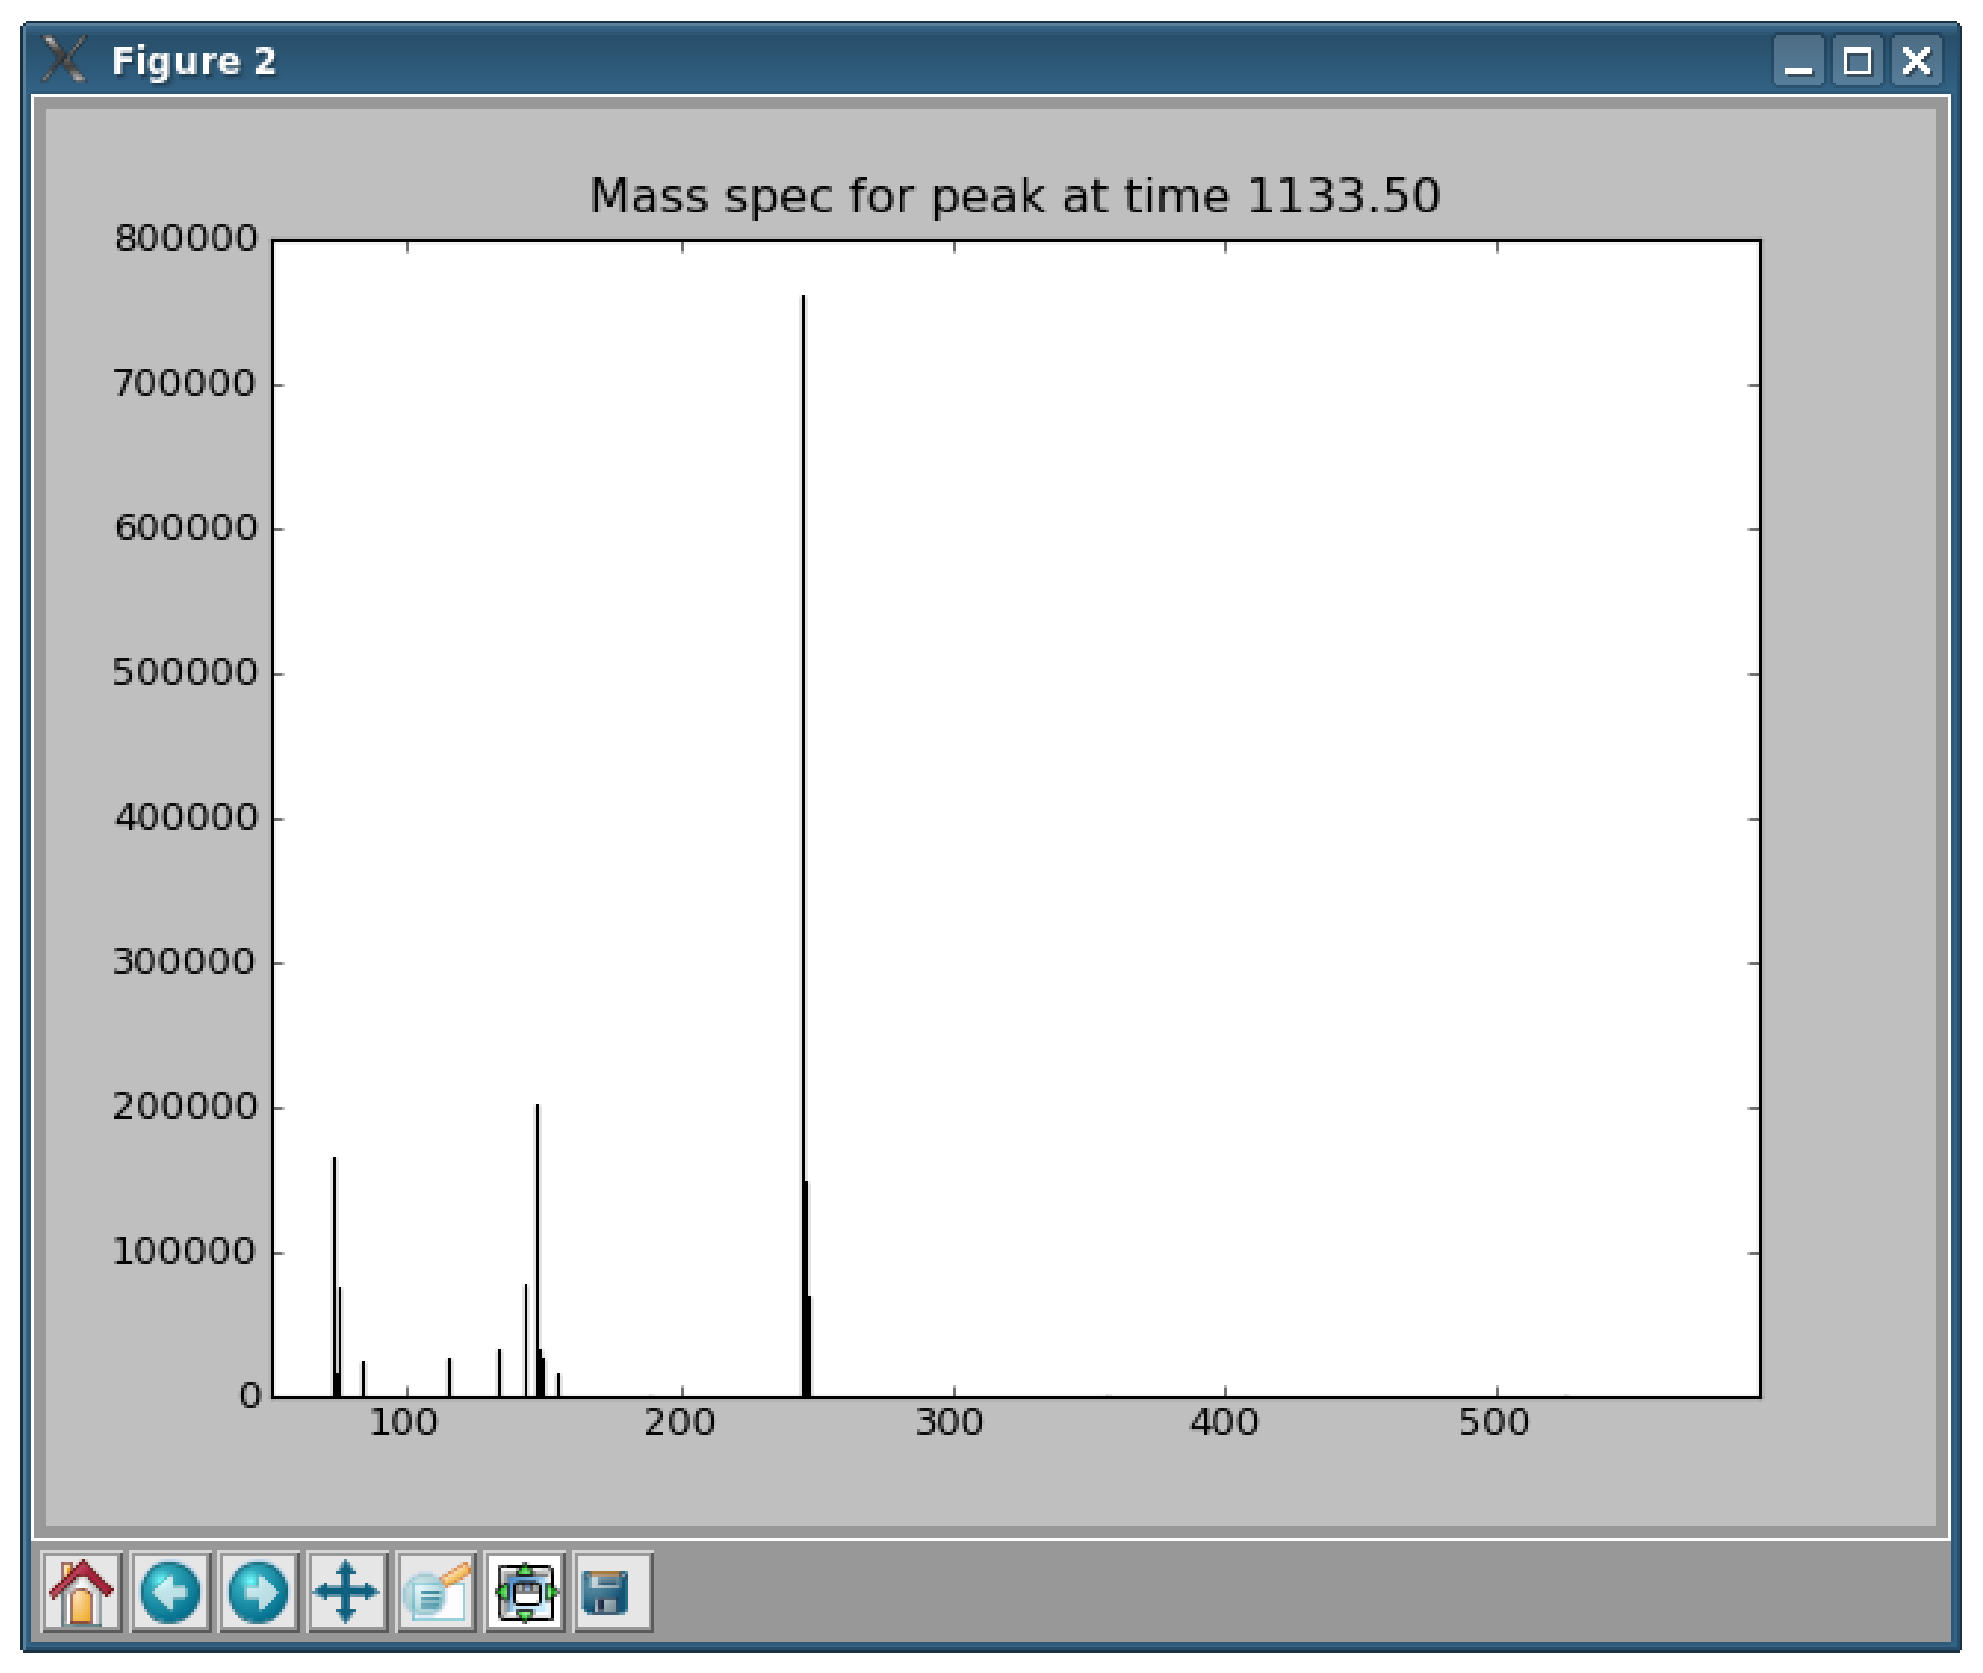
\includegraphics[scale=0.33]{graphics/chapter07/test-71-spec.eps}
  \end{center}
  \caption{The mass spectrum displayed by PyMS when a peak in the
  graphics window of Figure \ref{fig:71-ics} is clicked on}
  \label{fig:71-spec}
\end{figure}

Clicking on other peaks will display further mass spectrums for those peaks
in new windows.



%\setcounter{chapter}{8}
%\setcounter{section}{0}
%\pagenumbering{arabic}
% chapter08.tex

 %%%%%%%%%%%%%%%%%%%%%%%%%%%%%%%%%%%%%%%%%%%%%%%%%%%%%%%%%%%%%%%%%%%%%%%%%%%%%
 %                                                                           %
 %    PyMS documentation                                                     %
 %    Copyright (C) 2005-2010 Vladimir Likic                                 %
 %                                                                           %
 %    The files in this directory provided under the Creative Commons        %
 %    Attribution-NonCommercial-NoDerivs 2.1 Australia license               %
 %    http://creativecommons.org/licenses/by-nc-nd/2.1/au/                   %
 %    See the file license.txt                                               %
 %                                                                           %
 %%%%%%%%%%%%%%%%%%%%%%%%%%%%%%%%%%%%%%%%%%%%%%%%%%%%%%%%%%%%%%%%%%%%%%%%%%%%%

\chapter{Labelled data related algorithms}


\section
{Mass Isotopomer Distribution Extraction in $^{13}$C Labelling Experiments}

\noindent
[ \emph{This example is in pyms-test/91} ]

The aim of the algorithm is to alleviate manual data processing bottleneck by 
semi-automatically computing the mass isotopomer distribution (MID) of each 
metabolite of interest from raw GC-MS data files. MID is a direct measure of the
 metabolite's labelling pattern, and thus of great interest in carbon labelling 
 experiments as well as mathematical modelling of metabolic fluxes.

A metabolite with n carbon atoms can be labelled at any position resulting in
2$^{n}$ different combinations, which are called isotopomers. For example, 
if a metabolite contains three carbon atoms and we denote unlabelled atom with
 ‘0’ and labelled with ‘1’, the possible labelling patterns for the carbon 
backbone are 000, 001, 010, 011, 100, 101, 110, 111. Mass spectrometry can only
resolve isotopomer distribution completely if enough fragments can be detected 
(for a compound with n carbon atoms this means 2$^{n}$ – 1 different fragments 
containing different number and/or combinations of carbons).

The same metabolite has n+1 different masses: base mass M (000), singly labelled
mass M+1 (001, 010, 100), doubly labelled mass M+2 (011, 101, 110) and fully 
labelled mass M+3 (111). The MS measurement of the molecular ion, or any other 
fragment ion incorporating whole carbon backbone,  gives the mass isotopomer 
distribution (i.e. normalised M, M+1, M+2, M+3 values) of the compound.

GC-MS data pre-processing (high and low frequency noise removal) as well as the 
construction of Intensity Matrix is accomplished via functionality of the GCMS 
module( Figure \ref{fig:81}). The new algorithm takes a list of each 
metabolite’s fragment ions, TIC retention time and a required number of 
isotopomers (or MID vector size) and extracts the mass isotopomer distribution 
for each metabolite. The algorithm’s performance for a particular data set is 
optimised via two parameters, namely an intensity threshold and a time window.

\begin{figure}
  \begin{center}
    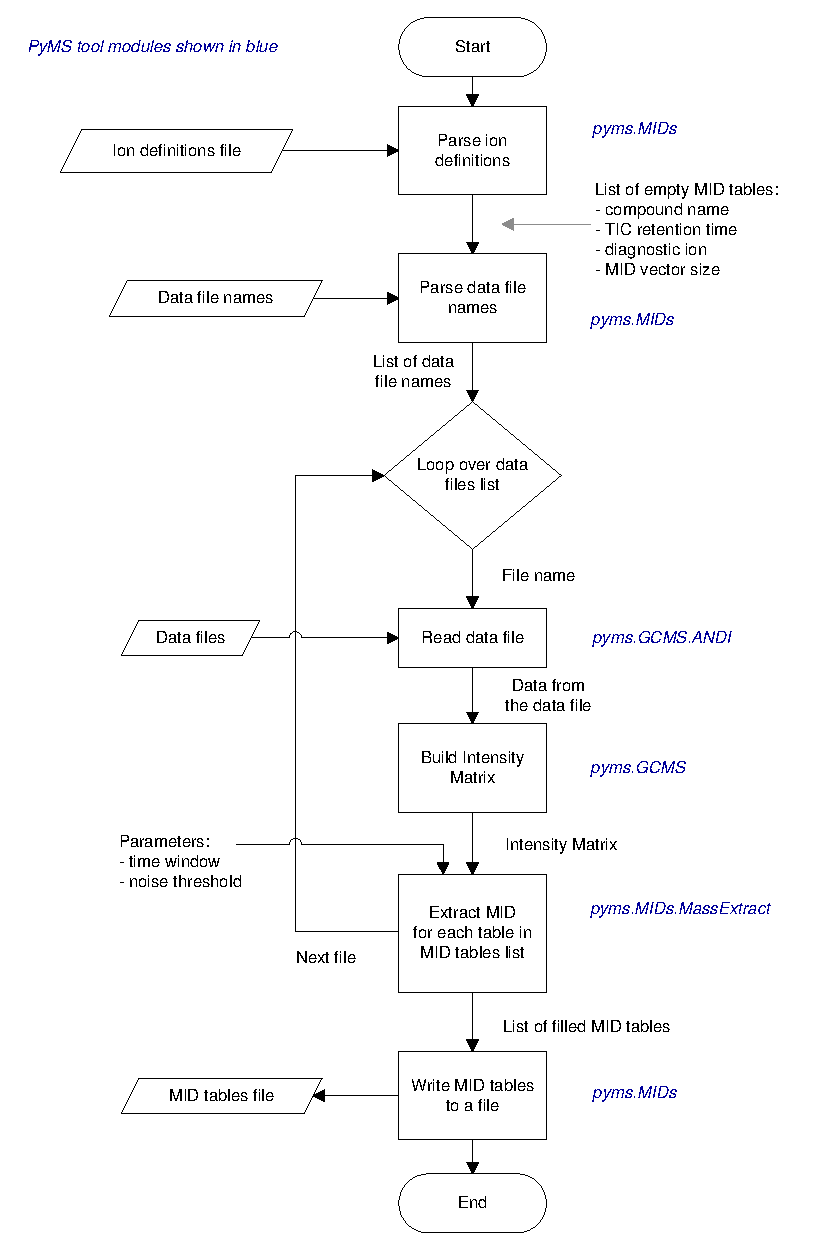
\includegraphics[scale=1]{graphics/chapter08/81.eps}
  \end{center}
  \caption{Data Flow Chart}
  \label{fig:81}
\end{figure}

In the example, experimental data are saved as a series of .CDF files, and the base 
file name is:
\begin{verbatim}
 '/x/PyMS/data/'
\end{verbatim}

The extension file numbers 'a20090\_3297', 'a200903\_298' and 'a200903\_299' are stored inside
'data\_files' file. The compound is alanine, the retention time is 6.93 minutes 
and the diagnostic ions are 190 and 116 with MID vector size of 6 (i.e. ions to 
be extracted are m/z 190, 191, 192, 193, 194, and 195 and 116, 117, 118, 119, 
120 and 121 respectively). This information is stored inside 'ion\_definitions' 
file.

To enter the input data:

\begin{verbatim}
>>> data_file_root = '/x/PyMS/data/'
>>> ion_defs = 'input/ion_definitions'
>>> data_defs = 'input/data_files'
>>> out_file = 'output/out.csv'
\end{verbatim}

Time window size used is 4 seconds, and intensity threshold is 4000. To enter 
both parameters:

\begin{verbatim} 
>>> time_win = 4 
>>> int_tresh = 4000 
\end{verbatim}

Then read in both input files:
\begin{verbatim}
>>> mid_table_list = parse_ion_defs(ion_defs)
>>> data_files = parse_data_defs(data_defs
\end{verbatim}

Next loop over data files and extract MID:
\begin{verbatim}
>>> for file_name in data_files:
>>>     andi_file = data_file_root + file_name + ".CDF"
>>>     data = ANDI_reader(andi_file)
>>>     im = build_intensity_matrix_i(data)
>>>     for mid_table in mid_table_list:
>>>         extract_mid(mid_table, file_name, im, time_win, int_tresh)
\end{verbatim}

Finally, write MID data tables to previously defined out\_file:
\begin{verbatim}
>>> write_mid_tables(mid_table_list, out_file)
\end{verbatim}

The out\_file should contain:

\begin{verbatim}

\end{verbatim}

\section
{MID Extraction - Algorithm Details}

\noindent

The overall information, and therefore possible inputs, available for each metabolite consists of:
- Diagnostic fragment ion value (e.g. m/z 116 for alanine) and a number of subsequent isotopomers
- TIC retention time from an unlabelled sample (e.g. 6.93 minutes)
- Chromatographic peak shape
- Unlabelled mass spectra

Next each of the above inputs and its implemented, as well as possible, use is considered in detailed.

\subsection
{Diagnostic Ion Value and Number of Mass Isotopomers}
The fragment ion value is used to extract Ion Chromatogram of the unlabelled 
isotopomer as well as subsequent, labelled, isotopomers, the number of which is 
predetermined. This information is constant and does not change across files. 
For example, in case of alanine fragment m/z 116, which contains 2 backbone 
carbons, there are 2 subsequent isotopomers m/z 117 (contains singly labelled 
carbon) and m/z 118 (contains two labelled carbons). Since we are dealing with 
metabolically labelled data, carbons belonging to the derivatisation agent are 
considered unlabelled (this is not strictly true due to natural isotopic 
abundance - dealt with in the next section).  Another important point is that 
each compound will have many fragments containing both different and the same 
parts of the carbon skeleton, thus redundant data will be available for 
consistency checks. These checks are currently not implemented. A further study 
should be conducted to determine, which fragments contain the same information 
and which ones can be used for redundancy checks (the fragment usability will 
depend on co-elution and relative abundance).

Example in the figure \ref{fig:82} gives a visual representation of the 
extraction of m/z 116 diagnostic ion for TMS derivatised alanine. The 
subsequent isotopomer ICs are extracted in the likewise manner.

\begin{figure}
  \begin{center}
    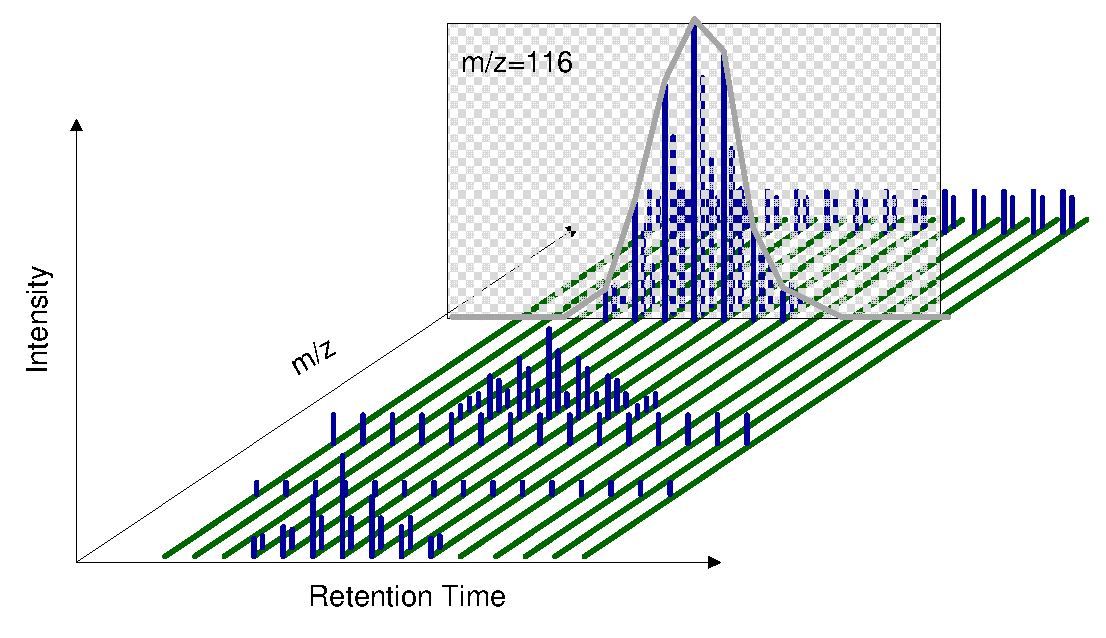
\includegraphics[scale=0.7]{graphics/chapter08/82.eps}
  \end{center}
  \caption{Ion Chromatogram Extraction at m/z 116}
  \label{fig:82}
\end{figure}

\subsection
{TIC Retention Time}
Unlike the fragment ion value, the use of TIC retention time is less dependable. 
In the current processing procedure, retention time value must be manually 
obtained from an unlabelled standard (once for each metabolite) at the 
beginning of each experiment run. TIC retention time is prone to change with 
the settings of the GC-MS instrument (e.g. pressure, temperature) as well as 
normal operating conditions (e.g. cutting of the GC column). Retention time 
locking and use of retention indices have both been developed to counteract 
this inherent time shift. 

The GC-MS instrument is capable of adjusting pressure to lock one compound to a 
particular retention time. This means that a particular compound can be chosen 
to elute at an exact time. For example, mannitol can be chosen to elute 
at 10.5mins every time. Mannitol is chosen for the fact that its retention time 
is in the middle of most metabolomic TICs, thus giving the maximum benefit (as 
opposed to choosing the compound at the beginning or end of a TIC). This 
procedure is referred to as retention time locking.

While the retention time locking aims to eliminate the effect of the linear 
component of the retention time drift, indices aim to compensate for the 
non-linear time shift (i.e. TIC expansion and contraction). Ideally, a group 
of alkines each differing by 2 carbon atoms (e.g. C10 to C32) is added to 
samples. The alkines elute in an equidistant pattern, and are given indices of 
1000, 1200, …, 3200. The components of interest are then assigned indices 
depending on their elution time relative to their two neighbouring alkines. For 
example, if a compound elutes ¼ of the way between alkine with 10 carbon atoms 
and alkine with 12 carbon atoms then its index is 1050. This is referred to as 
indices procedure.

Finally, as TIC retention time at peak apex will, most of the time, not be i
dentical to an IC retention time anyway, the algorithm has been designed to 
cope with a small variation in supplied retention time value. Thus, the 
retention time locking, currently employed in the local lab, is sufficient 
for its correct operation, and indices, while certainly beneficial, are not 
necessary.

\subsection{Peak Shape}

{\bf Detecting Peak Apex}

Following from the TIC retention time discussion in the previous section, the 
two anticipated scenarios are represented in figure \ref{fig:83}. The TIC retention 
time will be located immediately before (on the left of) or after 
(on the right of) IC’s peak apex.

\begin{figure}
  \begin{center}
    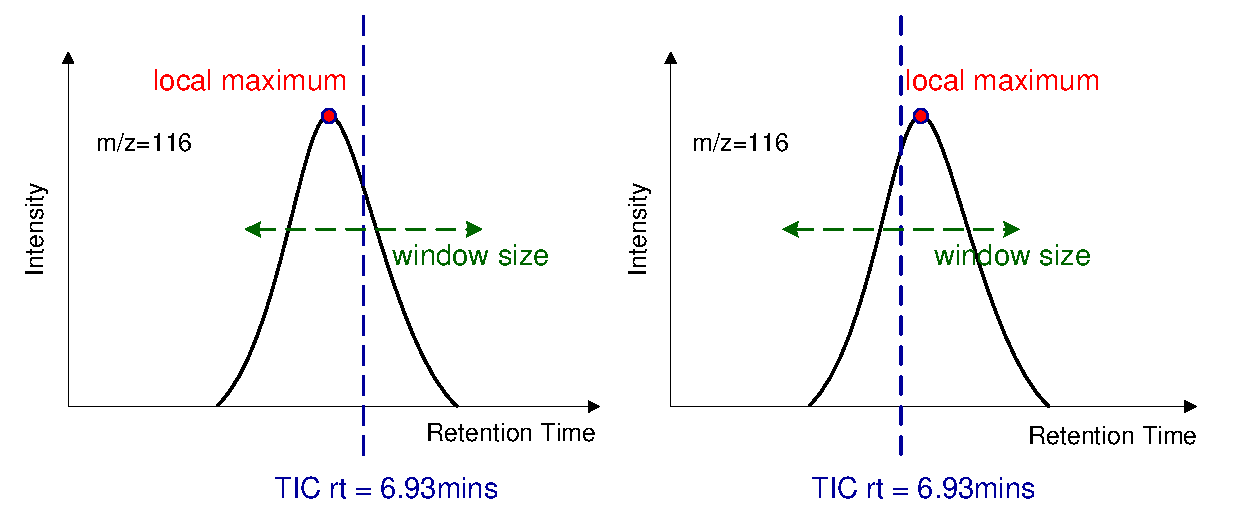
\includegraphics[scale=0.7]{graphics/chapter08/83.eps}
  \end{center}
  \caption{Peak Apex Detection}
  \label{fig:83}
\end{figure}


IC’s peak apex is then detected as a local maximum within a specified window. 
Time window size is a parameter set to just below average peak width. Too narrow 
window will fail to account for the time drift present and encompass the actual 
peak apex, and too wide window size will raise the probability of reaching the 
neighbouring peak apex instead. Both scenarios are discussed in detail next. 

As we are not guaranteed that the TIC retention time will be located within a 
specified window of ICs peak apex, and by examining the two dimensional IC 
space by placing our detected ‘local maximum’ at the origin of a Cartesian 
coordinate system, we can draw some conclusions on the success of finding the 
true peak apex (figure \ref{fig:84}). Firstly, if either left or right neighbouring intensities are 
greater than our detected ‘local maximum’ we can safely deduce that the IC peak 
apex detection has failed. In the case that both left and right neighbour 
intensities are equal a warning will be raised as GC-MS peaks are not expected 
to be flat, and this could indicate unusually high baseline. This can be further 
checked by comparing peak apex intensity with the instrument detection limit 
value (not implemented in the current version).

\begin{figure}
  \begin{center}
    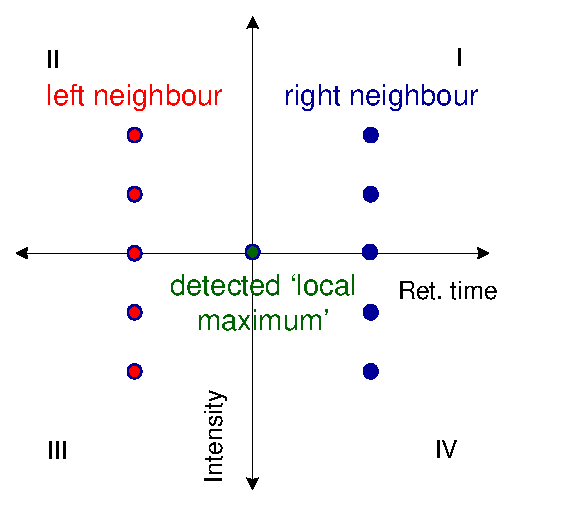
\includegraphics[scale=0.7]{graphics/chapter08/84.eps}
  \end{center}
  \caption{Left and Right Peak Neighbour Check}
  \label{fig:84}
\end{figure}

The above analysis also covers the scenarios where TIC retention time is located 
too close to a much larger peak, or the peak is simply missed by the particular 
IC retention time being too far to the left or too far to the right from the 
supplied overall TIC retention time (figure \ref{fig:85}).

\begin{figure}
  \begin{center}
    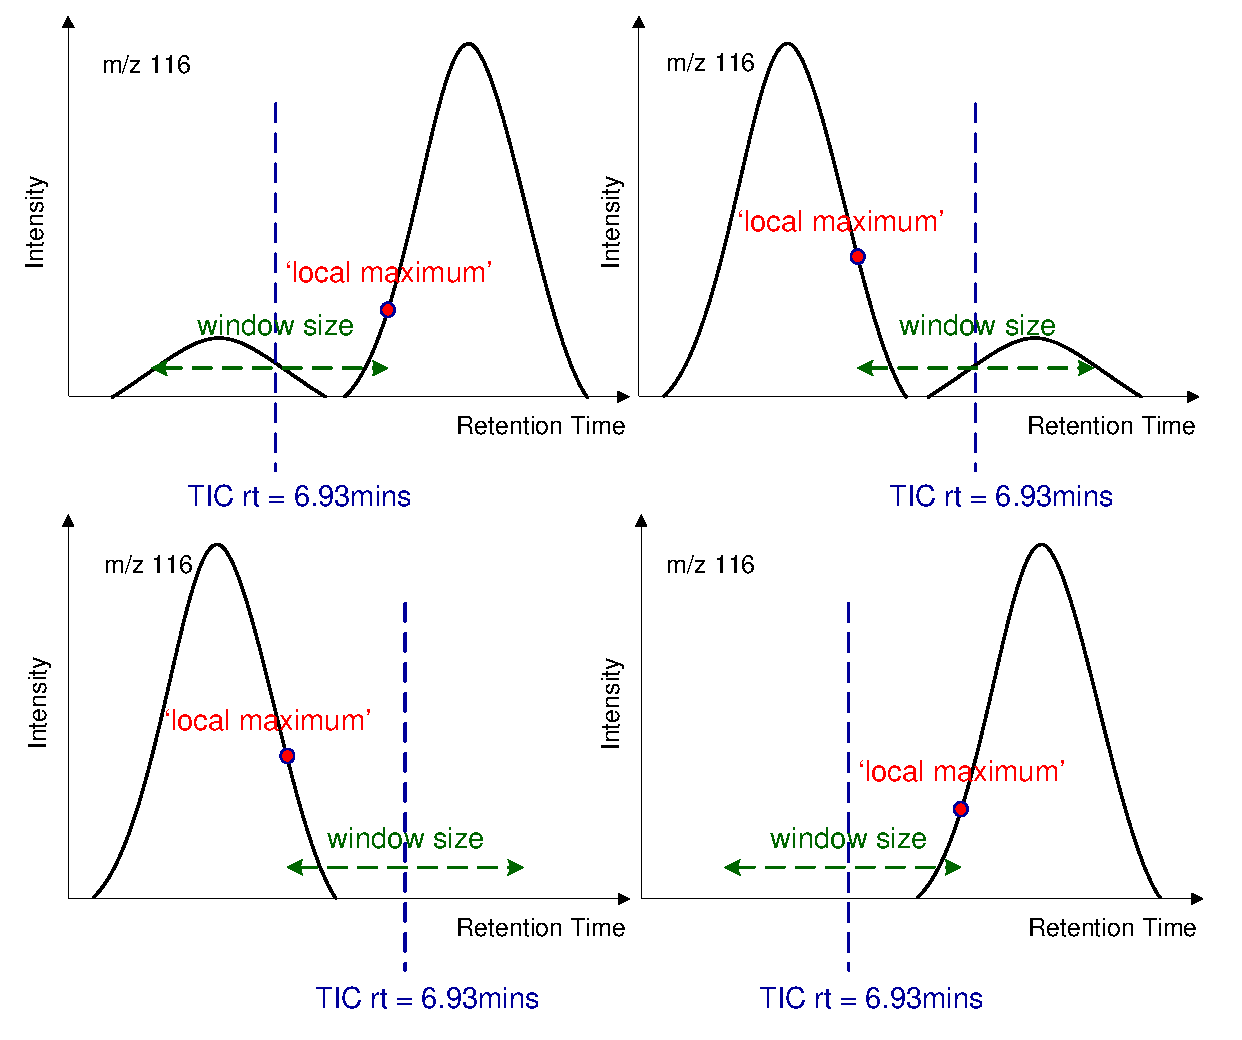
\includegraphics[scale=0.7]{graphics/chapter08/85.eps}
  \end{center}
  \caption{Missed or Large Peak Check}
  \label{fig:85}
\end{figure}

The four scenarios pictured in figure \ref{fig:85} suggest a fifth ‘middle 
ground’ scenario shown in figure \ref{fig:86}. Namely TIC retention time can 
land in the middle of two peaks with similar intensities. With only a slight 
time shift between ICs the detected peak apex could oscillate between the two 
peaks! The algorithm will detect this and raise a warning, as it is still 
possible to have an unusually wide peak with legitimate peak apex shift of 
plus/minus half the time window size (also pictured to the right). Note that 
the peaks in the first diagram in Figure 16 belong to the same IC, while the 
two peaks in the diagram on the right belong to two different ICs.

\begin{figure}
  \begin{center}
    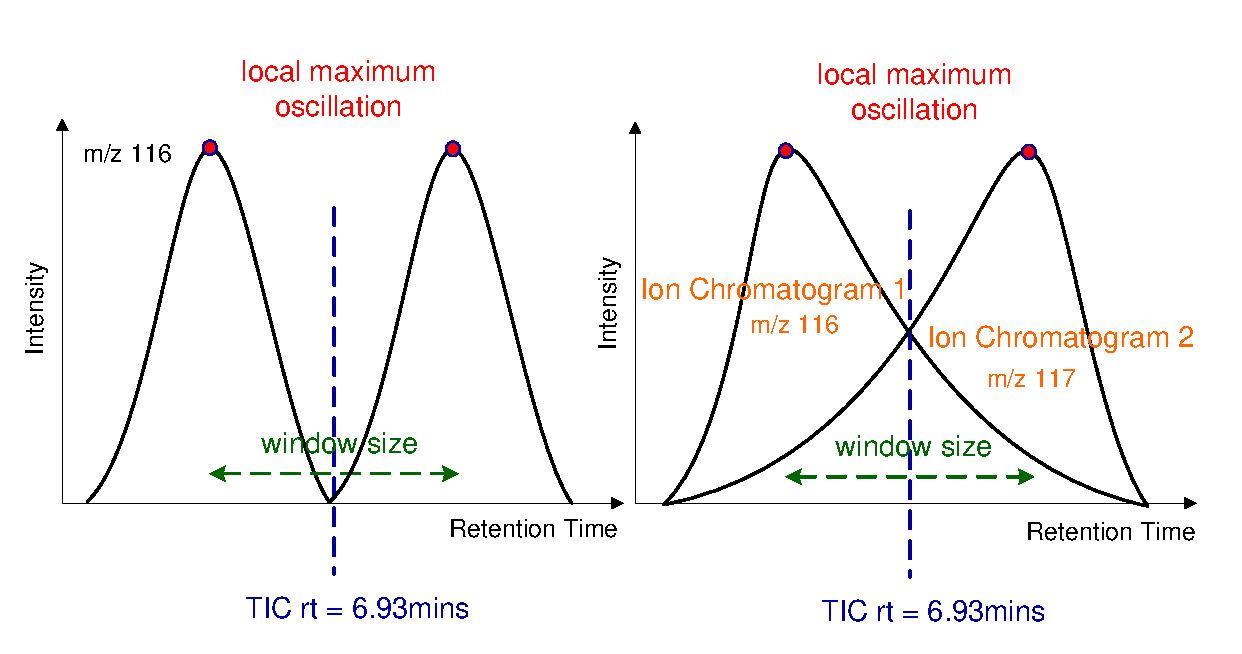
\includegraphics[scale=0.7]{graphics/chapter08/86.eps}
  \end{center}
  \caption{Close or Wide Peak}
  \label{fig:86}
\end{figure}

{\bf Detecting left and right boundary}

Having analysed the possible scenarios for the relationship between TIC 
retention time and detected peak apex, this brings us to the detection of left 
and right peak boundary (figure \ref{fig:87}). If our peak detection was 
successful this should be as easy as detecting first local minimum on the right 
and first local minimum on the left of detected peak apex. The integration then 
proceeds via summing up of all intensity between the two boundaries.

\begin{figure}
  \begin{center}
    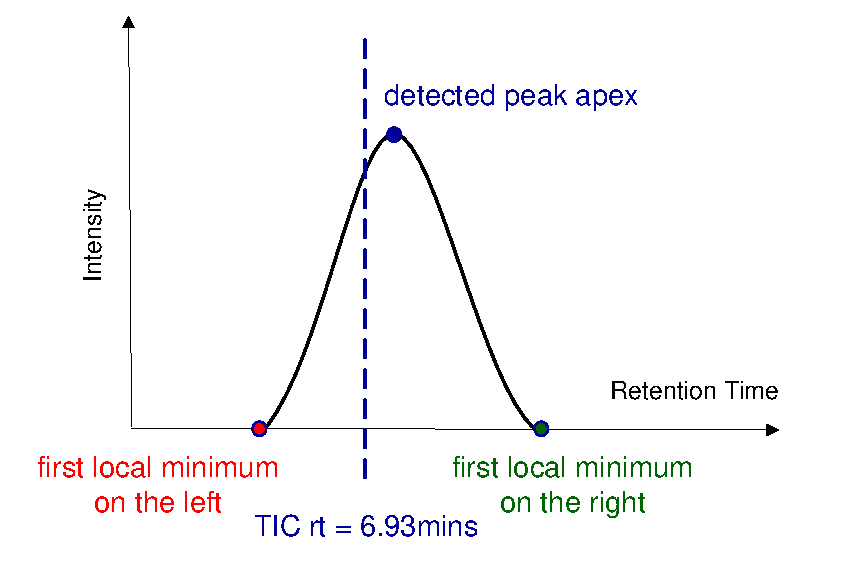
\includegraphics[scale=0.7]{graphics/chapter08/87.eps}
  \end{center}
  \caption{Feature detection at mass-to-charge ratio of 116 and retention time of 6.93 minutes}
  \label{fig:87}
\end{figure}

In addition integrating multiple ICs belonging to a single compound inside a 
single file can help integrate low intensity irregular shape peaks. This is 
pictured in figure \ref{fig:88}, and accomplished via setting an intensity 
threshold parameter which is equal to the intensity below which peaks are too 
close to the noise, irregular shape and impossible to integrate via above 
described method. In the drawing below the procedure is illustrated for the 
‘peak’ inside the IC belonging to the m/z of 119. Should there be no peaks with 
intensity above the threshold no integration occurs, should there be only a 
single peak above the threshold a warning is issued. The diagram also 
illustrates the importance of baseline correction for these low intensity peaks.

\begin{figure}
  \begin{center}
    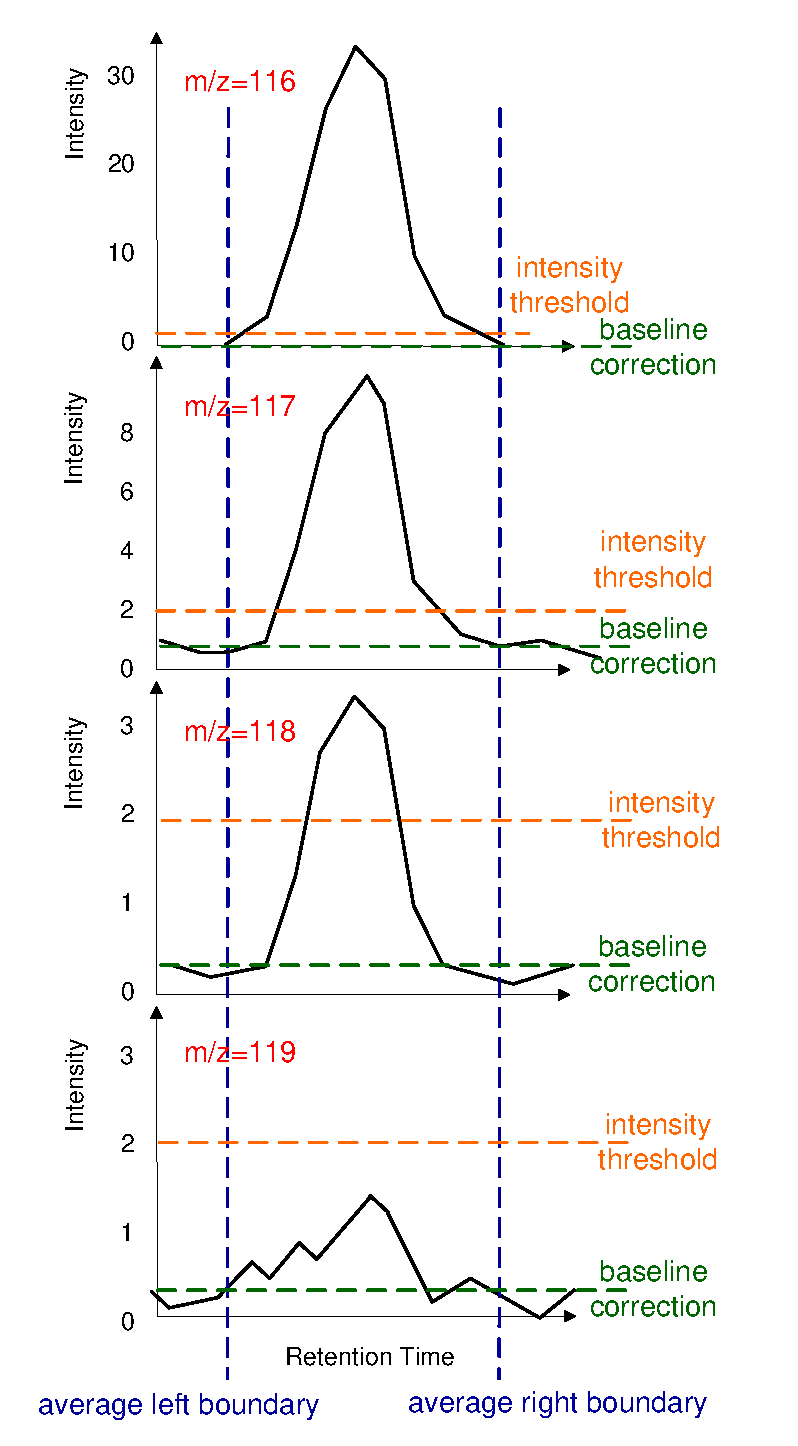
\includegraphics[scale=0.7]{graphics/chapter08/88.eps}
  \end{center}
  \caption{Averaging of left and right boundary values inside each Ion Chromatogram, and baseline correction (inspired by Antoniewicz et al., 2007a)}
  \label{fig:88}
\end{figure}

The introduction of an intensity threshold parameter introduces one more 
undesirable scenario. Namely, as peaks are not detected below threshold and the 
algorithm operates in a ‘blind mode’ it is possible for a neighbouring peak 
(not present or not as high intensity in other ICs) to interfere with the 
integration result (figure \ref{fig:89}). Should this happen a warning is raised.

\begin{figure}
  \begin{center}
    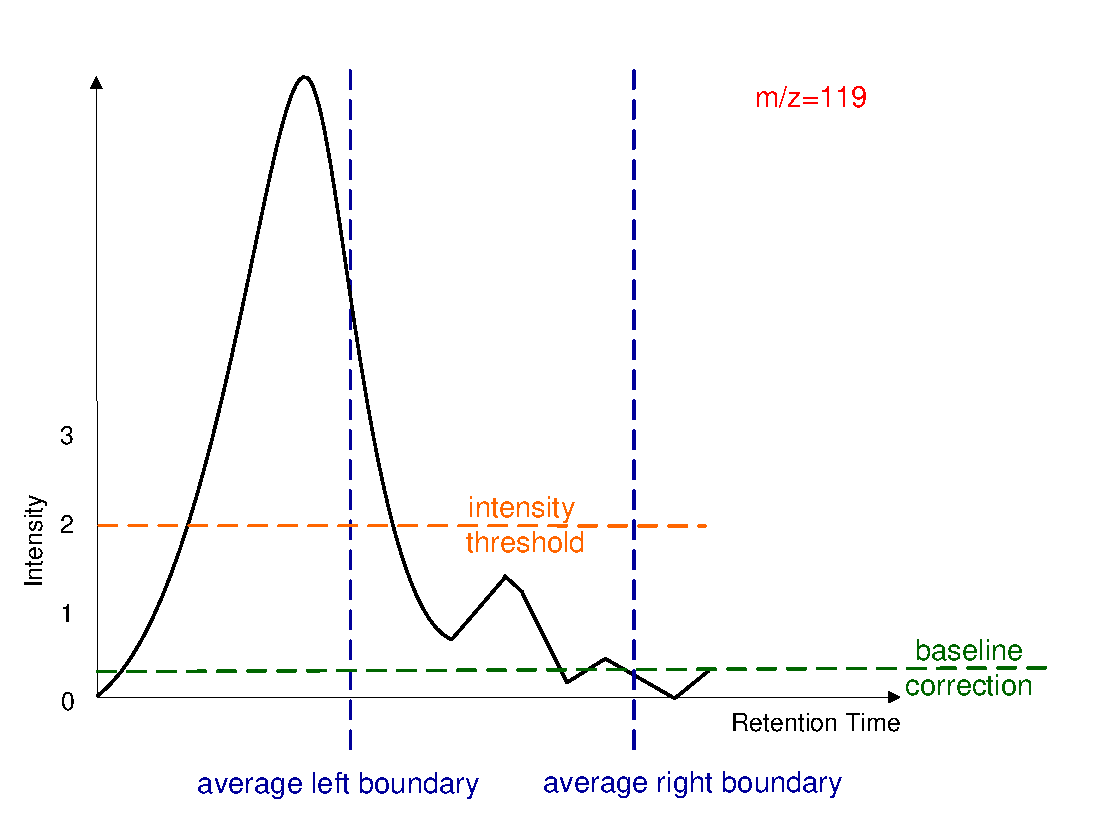
\includegraphics[scale=0.7]{graphics/chapter08/89.eps}
  \end{center}
  \caption{Large Peak Co-eluting with a Peak below Intensity Threshold}
  \label{fig:89}
\end{figure}

\subsection
{Mass Spectra}

The diagram in Figure \ref{fig:89} introduces another important question. 
When is a neighbouring peak a co-elution and when just a shoulder? The only way 
to reliably distinguish the two scenarios is via the use of mass spectra, which 
acts as a signature for a particular compound in GC-MS data. In fact TIC 
retention time itself is determined via mass spectral library, which can be 
used inside unlabelled data. Metabolic labelling, however introduces uncertainty 
into this signature, i.e. components can no longer be compared with the standard 
unlabelled mass spectra. Indeed, a test run of an existing similarity algorithm 
(Robinson et al., 2007) showed that labelled mass spectra can be more similar 
to spectra of other labelled compounds, than their own unlabelled spectra.

\begin{figure}
  \begin{center}
    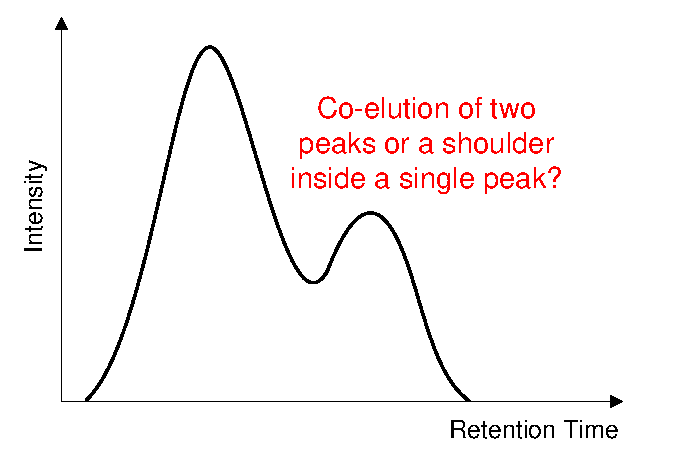
\includegraphics[scale=0.7]{graphics/chapter08/90.eps}
  \end{center}
  \caption{Co-elution or a Shoulder of a Single Peak Dilemma}
  \label{fig:90}
\end{figure}

However, we speculate that it might be possible to use a mass spectrum at peak 
apex inside labelled data to at least run a check between, and just outside, 
the integration boundaries. This might give an answer to a question if we have 
missed a shoulder or included a neighbouring peak in the overall integration. 

The above will, of course, not solve the question of certainty that the right 
compound was integrated. In theory it should be possible to design an elaborate 
algorithm, which would compute all possibilities of metabolic labelling, as 
well as take natural isotopic abundance into account, and then score the 
probability of integrated peak belonging to the compound we were interested in. 
This is indeed what analysts do in practice. In the manual procedure unlabelled 
chromatogram is compared to a labelled chromatogram. At the apex of a peak, the 
mass spectral fingerprint of both labelled and unlabelled metabolites is 
compared by eye. Labelled metabolites are expected to result in an increase in 
the mass to charge ratio of ions in the labelled chromatogram, and based on the 
retention time and mass spectra similarity analyst decides if the peaks belong 
to the same compound or not. Therefore it is argued that, although outside the 
scope of this algorithm due to time constraint considerations, the process 
should be amenable to automation. 

\subsection
{Setting the two parameters}

Setting the threshold too high will result in large number of unintegrated 
peaks. Setting the threshold too low will result in the algorithm attempting 
to integrate irregular shaped peaks thus setting off a large amount of warnings 
indicative of false positives. Due to a large variety in the abundance of 
metabolites one could almost perform two runs: one for high abundance peaks 
with higher threshold (to avoid peak shape detection of dubious peaks), and one 
for low abundance peaks which would benefit from lower threshold. This of course 
is not necessary and a well-chosen single threshold is sufficient. 

As discussed earlier, setting the window size too narrow will result in 
inability to detect peak apex (as it will not be present within the window) 
setting the window too wide will increase the chance of neighbouring peak being 
detected instead. Thus a window size of just below average peak width will give 
optimum performance.

\section
{Mass Isotopomer Distribution Correction in $^{13}$C Experiments}

\noindent
[ \emph{This example is in pyms-test/92} ]

Method implemented is that of Wittman and Heinzle \cite{wittman99}, and the details
of the example are given in Nanchen et al \cite{nanchen07}. 

Higher mass ion intensities (M, M + 1, M + 2, etc.) from $^{13}$C tracer 
experiments will include natural abundance of non-C isotopes and also natural 
abundance of $^{13}$C isotopes inside the GC-MS derivatization reagent, if 
applicable. The function takes the experimental ion intensities, which are obtained 
prior via integration of individual ion chromatograms, calculates the corresponding 
mass distribution vector and performs the correction  for natural isotope 
abundances of C, O, N, H, Si, and S atoms, as well as any unlabelled biomass (this 
corrects for the fact that in practice substrate is never 100\%\ labelled). The 
result is a corrected mass distribution vector. Fractional labelling value is also
provided as a check, and it should be equal to the fractional labelling of the
input substrate.

Experimental data is entered using the 'mdv' variable. In the example of
alanine fragment (M-57)+ \cite{nanchen07} there are n = 3 exogenous (non-natural
abundance) C atoms, and the length of the mass distribution vector
is chosen to be n+1=4. Hence only first four intensities (ion counts)
from the mass spectrum, corresponding to M, M+1, M+2 and M+3, are entered.

\begin{verbatim}
>>> mdv = [737537, 179694, 88657, 178433]
>>> n = len(mdv) - 1
\end{verbatim}

Determine the number of C, O, N, H, Si, and S atoms in the fragment,
noting that the number of C atoms excludes C atoms which may contain
exogenous $^{13}$C atoms. For the alanine (M-57)+ fragment these
numbers are C=8, O=2, N=1, H=26, Si=2, and S=0.

\begin{verbatim} 
>>> atoms = { 'c':8, 'o':2, 'n':1, 'h':26, 'si':2, 's':0}
\end{verbatim}

Import the relevant modules:

\begin{verbatim}
>>> import numpy
>>> import pyms.LabelledData.MID.Correct.Function
>>> import pyms.LabelledData.MID.Correct.Constants
\end{verbatim}

Calculate the overall correction matrix:

\begin{verbatim}
>>> c_corr = pyms.LabelledData.MID.Correct.Function.overall_correction_matrix(n, mdv, atoms)

Calculating c correction matrix

Calculating h correction matrix

Calculating si correction matrix

Calculating o correction matrix

Calculating n correction matrix

Calculating s correction matrix

Calculated overall correction matrix.

>>> c_corr array([[0.77152972 , 0.         , 0.         , 0.        ],
                  [0.1508547  , 0.77152972 , 0.         , 0.        ],
                  [0.06721399 , 0.1508547  , 0.77152972 , 0.        ],
                  [0.00866575 , 0.06721399 , 0.1508547  , 0.77152972]])
\end{verbatim}

Calculate the exclusive mass isotope distribution of the carbon skeleton:

\begin{verbatim}
>>> mdv_alpha_star = pyms.LabelledData.MID.Correct.Function.c_mass_isotope_distr(mdv, c_corr)
>>> mdv_alpha_star array([[ 0.7729932 ],
                          [ 0.03719172],
                          [ 0.01830562],
                          [ 0.17150946]])
\end{verbatim}

Correct for unlabelled biomass. This example accounts for the contribution
of 1\%\ unlabelled biomass.

\begin{verbatim}
>>> f_unlablelled = 0.01 
>>> mdv_aa = pyms.LabelledData.MID.Correct.Function.corr_unlabelled(n, mdv_alpha_star, f_unlabelled)
>>> mdv_aa array([[ 0.77102099],
                  [ 0.03725005],
                  [ 0.01848709],
                  [ 0.17324187]])
\end{verbatim}

Calculate the fractional labelling:

\begin{verbatim}
>>> fl = pyms.LabelledData.MID.Correct.Function.fract_labelling(n, mdv_aa)
Fractional labelling FL: 0.197983278219
\end{verbatim}


%\setcounter{chapter}{9}
%\setcounter{section}{0}
%\pagenumbering{arabic}
% chapter09.tex

 %%%%%%%%%%%%%%%%%%%%%%%%%%%%%%%%%%%%%%%%%%%%%%%%%%%%%%%%%%%%%%%%%%%%%%%%%%%%%
 %                                                                           %
 %    PyMS documentation                                                     %
 %    Copyright (C) 2005-2010 Vladimir Likic                                 %
 %                                                                           %
 %    The files in this directory provided under the Creative Commons        %
 %    Attribution-NonCommercial-NoDerivs 2.1 Australia license               %
 %    http://creativecommons.org/licenses/by-nc-nd/2.1/au/                   %
 %    See the file license.txt                                               %
 %                                                                           %
 %%%%%%%%%%%%%%%%%%%%%%%%%%%%%%%%%%%%%%%%%%%%%%%%%%%%%%%%%%%%%%%%%%%%%%%%%%%%%

\chapter{Parallel processing with PyMS}

\section{\label{sec:mpi}Requirements}

Using PyMS parallel capabilities requires installation of the package
'mpi4py', which provides bindings of the Message Passing Interface (MPI)
for the Python programming language. This package can be downloaded
from {\tt http://code.google.com/p/mpi4py/}. Since 'mpi4py' provides
only Python bindings, it requires an MPI implementation. We recommend
using mpich2:\\
{\tt http://www.mcs.anl.gov/research/projects/mpich2/}\\
We show the installation of 'mpich2' and 'mpi2py' on Linux system from
software distributions downloaded from the projects' web site.

\subsection{\label{sec:mpich2}Installation of 'mpich2'}

\begin{enumerate}

\item From the mpich2 project web site download the current distribution of
mpich2 (in our case the file 'mpich2-1.2.1p1.tar.gz').

\item Prepare the directory for mpich2 installation. In this example
we have chosen to use /usr/local/mpich2/. Our version of mpitch2 is
1.2.1, and to allow for the installation of different version later,
we create a subdirectory "1.2.1",

\begin{verbatim}
$ mkdir -vp /usr/local/mpich2/1.2.1
\end{verbatim}

The above command will make the directory /usr/local/mpich2/ and also
/usr/local/mpich2/1.2.1. Note that /usr/local is usually owned by
root, and the above commands may require root privileges.

\item Unpack this file and change to the source code directory:

\begin{verbatim}
$ tar xvfz mpich2-1.2.1p1.tar.gz 
$ cd  mpich2-1.2.1p1
\end{verbatim}

\item Configure, compile, and install mpich2:

\begin{verbatim}
$ ./configure --prefix=/usr/local/mpich2/1.2.1 --enable-sharedlibs=gcc
$ make
$ make install
\end{verbatim}

If /usr/local/mpich2/1.2.1 is owned by rood, the above command
may require root privileges.

\end{enumerate}

\subsection{\label{sec:mpi4py}Installation of 'mpi4py'}

\begin{enumerate}

\item From the mpi4py project web site download the current distribution
of mpi4py (in our case the file 'mpi4py-1.2.1.tar.gz').

\item Unpack this file and change to the source code directory:

\begin{verbatim}
$ tar xvfz mpi4py-1.2.1.tar.gz
$ cd mpi4py-1.2.1
\end{verbatim}

\item Edit the file 'mpi.cfg' to reflect the location of mpich2.  In
our case this file after editing contained the following:

\begin{verbatim}
# MPICH2
[mpi]
mpi_dir              = /usr/local/mpich2/1.2.1
mpicc                = %(mpi_dir)s/bin/mpicc
mpicxx               = %(mpi_dir)s/bin/mpicxx
\end{verbatim}

\item Install mpi4py:

\begin{verbatim}
$ python setup.py install
\end{verbatim}

\item Check that mpi4py works:

\begin{verbatim}
$ python
Python 2.5.2 (r252:60911, Sep 10 2008, 14:39:22) 
[GCC 4.1.1 20070105 (Red Hat 4.1.1-52)] on linux2
Type "help", "copyright", "credits" or "license" for more information.
>>> import mpi4py
>>> 
\end{verbatim}

If the above command import produced no output, mpi4py is installed
properly and ready to use.

\end{enumerate}

\section{\label{sec:parallel-background}Background to using PyMS in parallel}

Any processing that loops through ion chromatograms or mass spectra can
be performed in parallel, by distributing the processing of individual
ion chromatograms or mass spectra to different CPUs by using the
efficient MPI mechanism.

Before the parallel processing can be deployed, data needs to be binned
to produce an IntensityMatrix object, as described in the Section
\ref{sec:intensity-matrix}. This is essentially a two dimensional
matrix, with ion chromatograms along one dimension and mass spectra
along the other dimension.

Consider the processing which applies a noise smoothing function to
each ion chromatogram. We first read the raw data:

\begin{verbatim}
andi_file = "/x/PyMS/data/gc01_0812_066.cdf"
data = ANDI_reader(andi_file)
\end{verbatim}
 
Then build the intensity matrix, and get its dimensions:

\begin{verbatim}
im = build_intensity_matrix_i(data)
n_scan, n_mz = im.get_size()
\end{verbatim}

The last command sets the variables n\_scan and n\_mz to the number
scans and number of m/z values present in data, respectively.
Processing of ion chromatograms with the noise smoothing function
requires fetching of each ion chromatogram from the data, and
application of the noise smoothing function. This can be achieved 
with a simple loop: 

\begin{verbatim}
for ii in n_mz:
    print ii+1,
    ic = im.get_ic_at_index(ii)
    ic_smooth = window_smooth(ic, window=7)
\end{verbatim}

This example epitomizes the typical processing required on the
GC-MS data. Another, equally important processing, is that of
individual mass spectra. In this case the same logic can be
applied, except that one would loop over the other dimension
of the IntensityMatrix object 'im'. That is, one would loop
over all the scan indices, and use the method 
get\_ms\_at\_index() to fetch individual mass spectra:


\begin{verbatim}
for ii in n_scan:
    print ii+1,
    ms = im.get_ms_at_index(ii)
    # here do something the the mass spectra 'ms'
\end{verbatim}

Processing of data in this fashion is computationally intensive.
A typical data set may consist of 3,000-10,000 scans and ~500
m/z values. If complex processing algorithms are applied to
each ion chromatogram (or mass spectra), the processing will
quickly become computationally prohibitive.

The type of calculation illustrated above is an ideal candidate
for parallelization because each ion chromatogram (or mass
spectrum) are processed independently. PyMS takes advantage
of this and allows one to harvest the power of multiple CPUs
to speed-up the processing. To achieve this PyMS can distributes
the loop from the above (either type, ie. over ion chromatograms
or mass spectra) over the available CPUs, achieving a linear
speed-up with the number of CPUs.


\section{\label{sec:parallel-pyms}Using PyMS in parallel}

Using PyMS in parallel requires a minimal intervention, only
that special method of the IntensityMatrix object is invoked
in the for loop described above. For looping over all ion
chromatograms in parallel,

\begin{verbatim}
for ii in im.iter_ic_indices():
    print ii+1,
    ic = im.get_ic_at_index(ii)
    ic_smooth = window_smooth(ic, window=7)
\end{verbatim}

The only change is that 

\begin{verbatim}
for ii in n_mz:
\end{verbatim}

is replaced with

\begin{verbatim}
for ii in im.iter_ic_indices()
\end{verbatim}

The corresponding method for looping over all mass spectra
would involve replacing:

\begin{verbatim}
for ii in n_scan:
\end{verbatim}

with

\begin{verbatim}
for ii in im.iter_ms_indices()
\end{verbatim}

The special constructs {\tt for ii in im.iter\_ic\_indices():} and
{\tt for ii in im.iter\_ms\_indices()} will distribute the calculation
in parallel if MPI capability is available (ie. mpi4py is installed
on the system, and multiple CPUs are available). If MPI capability
is not available, the processing will be performed in a serial mode.
Running in parallel also requires some prior preparations, as explained
below.

Consider how the following script that performs noise smoothing example
described above (named 'proc.py'). This script is can be run in serial
or parallel mode.

\begin{verbatim}
"""proc.py
"""

import sys
sys.path.append("/x/PyMS")

from pyms.GCMS.IO.ANDI.Function import ANDI_reader
from pyms.GCMS.Function import build_intensity_matrix_i
from pyms.Noise.Window import window_smooth

# read the raw data as a GCMS_data object
andi_file = "/x/PyMS/data/gc01_0812_066.cdf"
data = ANDI_reader(andi_file)

# build the intensity matrix
im = build_intensity_matrix_i(data)

# get the size of the intensity matrix
n_scan, n_mz = im.get_size()
print "Size of the intensity matrix is (n_scans, n_mz):", n_scan, n_mz

# loop over all m/z values, fetch the corresponding IC, and perform
# noise smoothing
for ii in im.iter_ic_indices():
    print ii+1,
    ic = im.get_ic_at_index(ii)
    ic_smooth = window_smooth(ic, window=7)
\end{verbatim}

A simple running of this script will produce a serial run without
any warning messages:

\begin{verbatim}
$ python proc.py
 -> Reading netCDF file '/x/PyMS/data/gc01_0812_066.cdf'
Size of the intensity matrix is (n_scans, n_mz): 9865 551
1 2 3 4 5 6 7 8 9 10 11 12 13 14 15 16 17 18 19 20 21 22 23 24 25
26 27 28 29 30 31 32 33 34 35 36 37 38 39 40 41 42 43 44 45 46 47
... [ further output deleted ] ...
\end{verbatim}

Inspection of the CPU usage during the execution of the program
shows that only one CPU is utilised 100\% (although multiple CPUs
are available) as shown in Figure \ref{fig:top-serial}.

\begin{figure}
  \begin{center}
    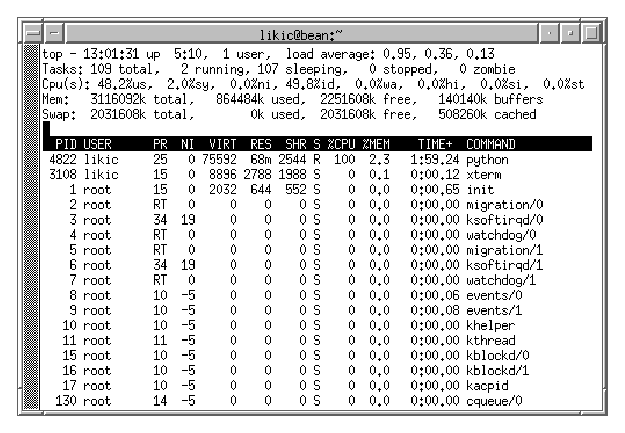
\includegraphics[scale=1.0]{graphics/chapter09/top-serial.eps}
  \end{center}
  \caption{The xterm output of the program 'top' with PyMS running in
  serial mode on the computer with multiple CPUs}
  \label{fig:top-serial}
\end{figure}

To run the above script in parallel, one needs first to start the
mpitch2 process launcher, called 'mpd' (this is a program, in this
example located in\\
 {\tt /usr/local/mpich2/1.2.1/bin/mpd},\\
see the section \label{sec:mpitch2}). This can be achieved as follows:

\begin{verbatim}
$ /usr/local/mpich2/1.2.1/bin/mpd --daemon
\end{verbatim}

The above command start 'mpd' as a daemon (the program runs in the
background, without a controlling terminal).  A common problem
that causes the above command is fail is the absence of the
{\tt .mpd.conf
\begin{figure}
  \begin{center}
    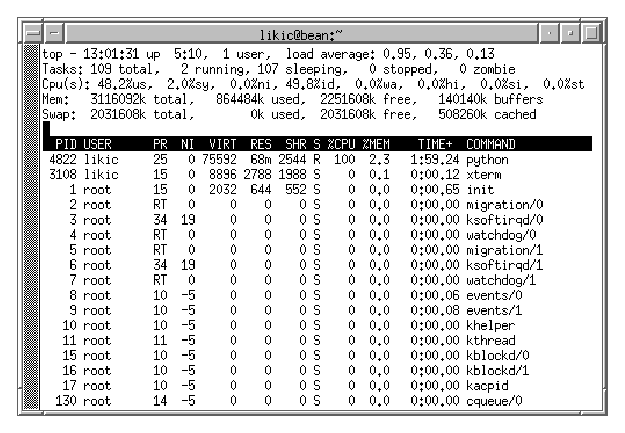
\includegraphics[scale=1.0]{graphics/chapter09/top-serial.eps}
  \end{center}
  \caption{The xterm output of the program 'top' with PyMS running in
  serial mode on the computer with multiple CPUs}
  \label{fig:top-serial}
\end{figure}
} file which 'mpd' requires to be present in the
home directory of the user who is starting the process. Here is
an excerpt from the 'mpd' help page:

\begin{verbatim}
A file named .mpd.conf file must be present in the user's home directory
with read and write access only for the user, and must contain at least
a line with MPD_SECRETWORD=<secretword>
To run mpd as root, install it while root and instead of a .mpd.conf file
use mpd.conf (no leading dot) in the /etc directory.' 
\end{verbatim}

Fixing this problem is simple, and requires creating the file
{\tt ~/.mpd.conf}, which in our case contains only one line:

\begin{verbatim}
MPD_SECRETWORD=euSe0veo
\end{verbatim}

After this the 'mpd' can be launched.  Running the PyMS script in the parallel
mode requires the use of 'mpirun' command,

\begin{verbatim}
$ /usr/local/mpich2/1.2.1/bin/mpirun -np 2 python proc.py 
\end{verbatim}

The above command prepare 'python proc.py' to run in parallel, in this
case by using two CPUS ({\tt -np 2}). The execution produces the
following output:

\begin{verbatim}
$ /usr/local/mpich2/1.2.1/bin/mpirun -np 2 python proc.py 
 -> Reading netCDF file '/x/PyMS/data/gc01_0812_066.cdf'
 -> Reading netCDF file '/x/PyMS/data/gc01_0812_066.cdf'
Size of the intensity matrix is (n_scans, n_mz):Size of
the intensity matrix is (n_scans, n_mz): 9865 551
276 9865 551
1 277 2 278 3 279 4 280 5 281 6 282 7 283 8 284 9 285 10 286 11 287 12
288 13 289 14 290 15 291 16 292 17 293 18 294 19 295 20 296 21 297 22
298 23 299 24 300 25 301 26 302 27 303 28 304 2
... [ further output deleted ] ...
\end{verbatim}

The above shows that two processes are active (each reading its own
version of data). While the distribution of processing between the
two processes has been achieved automatically by PyMS. Since both
processes were started from the same terminal their output is
intermingled. This time the processing is using two CPUs, and this
can be seen from the inspection of CPU utilisation, as shown in
Figure \ref{fig:top-parallel}. Also the execution of the script
'proc.py' is now two times faster.

\begin{figure}
  \begin{center}
    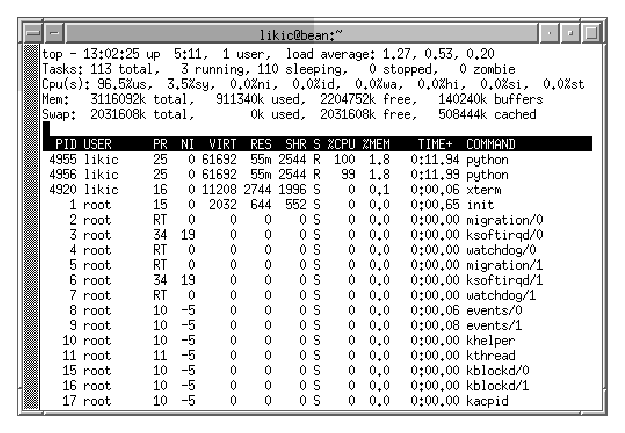
\includegraphics[scale=1.0]{graphics/chapter09/top-parallel.eps}
  \end{center}
  \caption{The xterm output of the program 'top' with PyMS running in
  parallel mode with two CPUs}
  \label{fig:top-parallel}
\end{figure}




\bibliography{bibtex/refbase}
\bibliographystyle{unsrt}

\backmatter
\printindex

\end{document}
